\documentclass{scrreprt}
%%\documentclass{scrbook}
\usepackage{lipsum}
%%\usepackage[french]{babel}
%%\usepackage[ngerman]{babel}


%% Choose default font for the document
%% Warning : only ONE of the following should be enabled
\usepackage{kpfonts}
%%\usepackage{libertine}

%% The following chose the default language for the document and
%% use the default typography rules for the choosen language.
\usepackage{polyglossia}
\setdefaultlanguage{english}
%% \setdefaultlanguage{german}
%%\setdefaultlanguage{french}

\usepackage[backend=biber, style=ieee]{biblatex}
\addbibresource{template.bib}

\usepackage{graphicx}
\graphicspath{ {./ressources/images/} }

\usepackage{markdown}
\usepackage{array}
\usepackage{appendix}

\usepackage{listings}
\usepackage{xcolor}
\definecolor{lightgray}{rgb}{.9,.9,.9}
\definecolor{darkgray}{rgb}{.4,.4,.4}
\definecolor{purple}{rgb}{0.65, 0.12, 0.82}
% Taken from Lena Herrmann at 
% http://lenaherrmann.net/2010/05/20/javascript-syntax-highlighting-in-the-latex-listings-package
\lstdefinelanguage{JavaScript}{
  keywords={typeof, new, true, false, catch, function, return, null, catch, switch, var, if, in, while, do, else, case, break},
  keywordstyle=\color{blue}\bfseries,
  ndkeywords={class, export, boolean, throw, implements, import, this},
  ndkeywordstyle=\color{darkgray}\bfseries,
  identifierstyle=\color{black},
  sensitive=false,
  comment=[l]{//},
  morecomment=[s]{/*}{*/},
  commentstyle=\color{purple}\ttfamily,
  stringstyle=\color{red}\ttfamily,
  morestring=[b]',
  morestring=[b]",
  columns=fullflexible,
  backgroundcolor = \color{lightgray}
}
% Taken from Edward Cooper at
% https://gist.github.com/ed-cooper/1927af4ccac39b083440d436d018d253
\definecolor{delim}{RGB}{20,105,176}
\definecolor{numb}{RGB}{106, 109, 32}
\definecolor{string}{rgb}{0.64,0.08,0.08}

\lstdefinelanguage{json}{
    numbers=left,
    numberstyle=\small,
    frame=single,
    rulecolor=\color{black},
    showspaces=false,
    showtabs=false,
    breaklines=true,
    postbreak=\raisebox{0ex}[0ex][0ex]{\ensuremath{\color{gray}\hookrightarrow\space}},
    breakatwhitespace=true,
    basicstyle=\ttfamily\small,
    upquote=true,
    morestring=[b]",
    stringstyle=\color{string},
    backgroundcolor = \color{lightgray},
    literate=
     *{0}{{{\color{numb}0}}}{1}
      {1}{{{\color{numb}1}}}{1}
      {2}{{{\color{numb}2}}}{1}
      {3}{{{\color{numb}3}}}{1}
      {4}{{{\color{numb}4}}}{1}
      {5}{{{\color{numb}5}}}{1}
      {6}{{{\color{numb}6}}}{1}
      {7}{{{\color{numb}7}}}{1}
      {8}{{{\color{numb}8}}}{1}
      {9}{{{\color{numb}9}}}{1}
      {\{}{{{\color{delim}{\{}}}}{1}
      {\}}{{{\color{delim}{\}}}}}{1}
      {[}{{{\color{delim}{[}}}}{1}
      {]}{{{\color{delim}{]}}}}{1},
}

\usepackage{pdfpages}
\usepackage{longtable}

\usepackage{hyperref}
\hypersetup{
    colorlinks=true, 
    linktoc=all,
    urlcolor     = black, %Colour for external hyperlinks
    linkcolor    = black, %Colour of internal links
    citecolor   = black %Colour of citations
}

\begin{document}

\begin{titlepage}
  \begin{center}
    {\LARGE \bfseries\sffamily Web Simulation of a Thymio Robot}
    \vspace{2mm}

    {\bfseries Bachelor thesis}
    \vspace{1cm}

    {\large Degree programme: Computer Science}
    \vspace{2mm}

    {\large Author: Quentin Flückiger (\texttt{flucq1@bfh.ch})}
    \vspace{2mm}

    {\large Thesis Advisor: Prof. Claude Fuhrer}
    \vspace{2mm}

    {\large Expert: Dr. Eric Dubuis}
    \vspace{2mm}

    \today
    \vspace{2cm}

    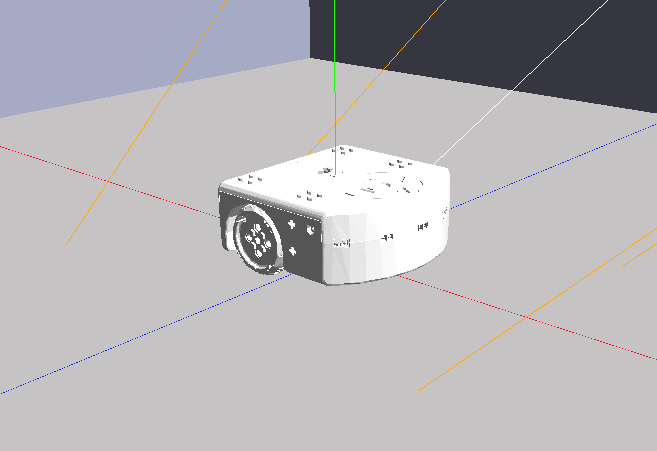
\includegraphics[width=\textwidth]{./title}
  \end{center}
\end{titlepage}

\clearpage

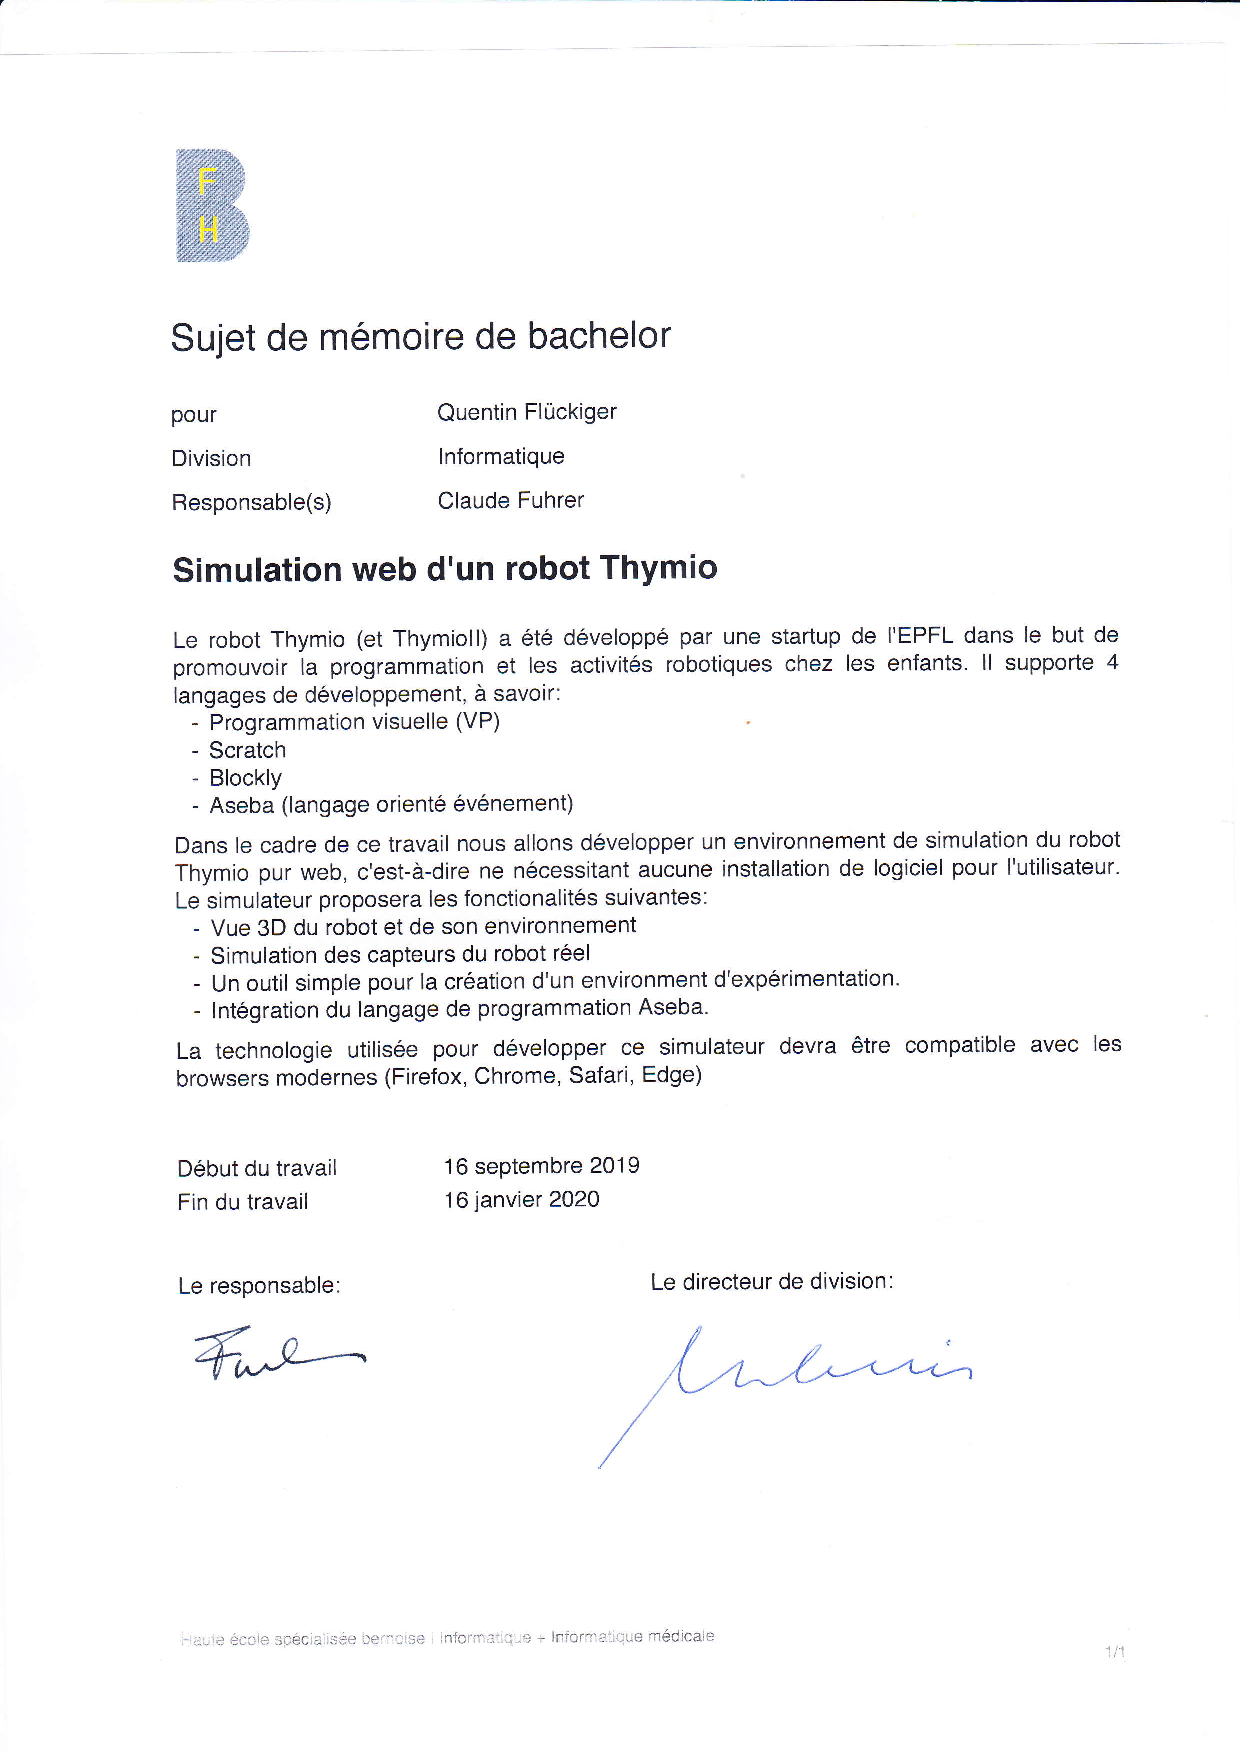
\includegraphics[width=\textwidth]{pdf/bachelor_quentin.pdf}
\clearpage

\section*{Management Summary}

As information technology has grown massively in everyday life during the last decade, many questions have arisen. A very important one, at the very least in our minds, concerns the educational side. 
To what extent should information technology be taught, in mandatory school, high school, vocational education, or even self-taught? In Switzerland, some optional courses in this field have already been introduced in the curriculum of some primary schools. 
Of course, the schoolkids are not taught too deep and complicated concepts, but they are rather familiarized with the way of reasoning and improving logical concepts. To ease the entry into the world of information technology, some schools have developed projects. 
One example is the Thymio project of the Swiss Federal Institute of Technology of Lausanne. Thymio is a small robot that can be programmed on a computer with four different languages, with varying degrees of difficulty. 
Thus, it allows very young people to experience and learn some of the basics of information technology. Unfortunately, this robot has a few disadvantages. One example is the space required or the setup of its environment. 
In order to fill these gaps, we have decided to create a simulation of the Thymio.
Therefore, the objective of this project is the creation of a Thymio simulator. The simulator has to be a web application to ease the accessibility, where no software installation is required, and it has to be compatible with modern browsers.

We started the project by learning about the four different languages supported by the robot, namely VPL, Blockly, Aseba, and Scratch. We were interested in knowing how to create a simple program with each of them and how the output programs were formatted. 
As we decided to make the simulator completely web, we needed a way to represent and animate computer graphic elements. In this sens, we chose \texttt{three.js} as a library.

Afterward, we created the base of the application. This base consists in loading a Thymio model and in having multiple basic playgrounds. On top of this we built a special playground creator tool, that allows the user to create his own playground with different meshes that he can place. 
The data are then stored inside a \texttt{JSON} file on the user's machine and they can be loaded in the simulator. The first actuator to be added, which is a component of a machine that is responsible for moving and controlling a mechanism or system, 
were the motors. We tried to make them behave as close to reality as possible, that is to say they can only do three things: move forward, move backward, or they do not move at all.

Last but not least, we had to develop a compiler that would translate a program written for Thymio in one of the four languages. In order to do this we used the code of the Thymio Suite application developed by \texttt{Aseba}. 
As their application was coded in \texttt{C++} it was needed to understand it and to translate them into \texttt{JavaScript}. 

\clearpage

\tableofcontents
\clearpage

\chapter{Requirements Documentation}
\section{Introduction}

As information technology has grown massively in everyday life during the last decade, many questions have arisen. A very important one, at the very least in our minds, concerns the educational side. 
To what extent should information technology be taught, in mandatory school, high school, vocational education, or even self-taught? In Switzerland, some optional courses in this field have already been introduced in the curriculum of some primary schools. 
Of course, the schoolkids are not taught too deep and complicated concepts, but they are rather familiarized with the way of reasoning and improving logical concepts. To ease the entry into the world of information technology, some schools have developed projects. 

\section{Vision}

The Thymio robot or Thymio II is a robot developed by a start-up from the EPFL in order to promote programming and robotic activities among children. 
To feed program to the robot, a software has been developed. It integrates the four following programming languages: 
\begin{itemize}
  \item VPL
  \item Blockly4Thymio
  \item Aseba
  \item Scratch
\end{itemize}

The project Web Simulation of a Thymio robot aims at creating a simulator for the Thymio II so as to allow people to directly see their programmed behavior.

\section{Goals}

This aim was split into 6 different defining goals in order to create this application.

\begin{center}
  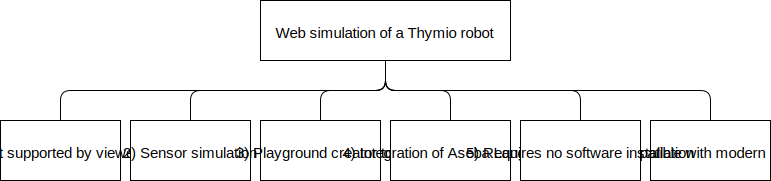
\includegraphics[width=\textwidth]{./goals}
\end{center}

\section{Risk Analysis}
In order to carry out the project successfully, one must consider several possible complications. These are on one hand assessed according to their impact and on the other hand according to their likelihood to occur. 
Thus, we obtain a predictable risk factor that allows us to have an overall view and take preventive measures if necessary.

\begin{center}
  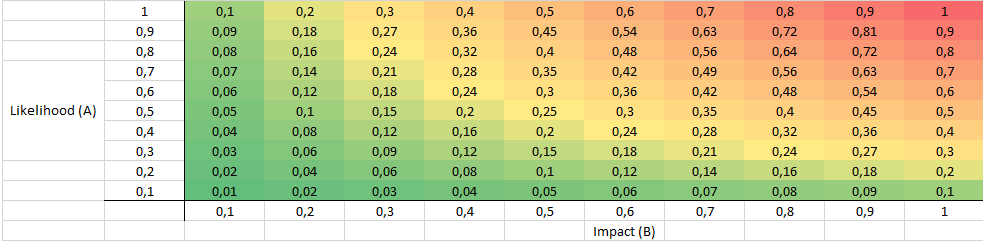
\includegraphics[width=\textwidth]{./risk-matrix}\\
  Risk Matrix
\end{center}

\begin{tabular}{p{2cm} p{2cm} p{2cm} p{2cm}}
  Event & Likelihood (A) & Impact (B) & Risk Factor (A*B) \\ \hline
  Financial issues & 0 & 1 & 0 \\
  Collisions not implemented & 0.3 & 0.6 & 0.18 \\
  Behavior pipeline not working & 0.4 & 0.9 & 0.36 \\
  Playground creator not working & 0.4 & 0.6 & 0.24 \\
\end{tabular}

\section{Stakeholder Descriptions}
\textbf{Product Owner}
Flückiger Quentin flucq1@bfh.ch \\
\textit{Interests}:
\begin{itemize}
  \item The product owner wants to satisfy the customer.
\end{itemize}


\textbf{Development Team}
Flückiger Quentin flucq1@bfh.ch \\
\textit{Interests}:
\begin{itemize}
  \item The development team wants to develop a usefull application for the customer.
\end{itemize}

\section{User Stories}
\textbf{\large Users User Stories}\\
\textbf{As} a user, I want to upload an .aesl file, so that I can witness the simulated behavior. \\
Description:\\
The user wants to upload an .aesl file to see the programmed behavior simulated.
Success:\\
\begin{itemize}
  \item The simulation works.
\end{itemize}
Failure:\\
\begin{itemize}
  \item The .aesl file does not contain a program.
  \item The .aesl file contains behavior not included in the simulator.
\end{itemize}


\textbf{As} a user, I want to create a simple testing environment, so that I can diversify the experiences. \\
Description:\\
The user wants to create a home made playground with a simple playground creation tool.
Success:\\
\begin{itemize}
  \item The playground is successfully created and saved.
\end{itemize}
Failure:\\
\begin{itemize}
  \item The created playground is not saved properly.
  \item The user encounters trouble while creating the playground, be it meshes creation or placement.
\end{itemize}


\textbf{As} a user, I want to use the application without having to install anything, so that the application can be accessed easily. \\
Description:\\
The user wants to access and use the application without installing anything.
Success:\\
\begin{itemize}
  \item The use can start the application directly in his browser.
\end{itemize}
Failure:\\
\begin{itemize}
  \item The webserver is not accessible.
\end{itemize}

\section{Use Cases Model}

\textbf{Use Case: }Access the application \\
\textbf{Primary Actor: }User \\
\textbf{Stakeholders and Interests: }User: Wants to access the application through a web browser. \\
\textbf{Preconditions: }User has access to the bfh network. \\
\textbf{Success Guarantee (Postconditions): }The user can access the application via a modern web browser. \\
\textbf{Main Success Scenario: } 
\begin{enumerate}
  \item User starts the web browser.
  \item User navigates to the website address.
\end{enumerate}
\textbf{Extensions: } 
\begin{enumerate}
  \item 
  \begin{enumerate}
    \item No available internet connection.
  \end{enumerate}
  \item 
  \begin{enumerate}
    \item Not logged in the bfh network.
    \item Web Server currently offline.
  \end{enumerate}
\end{enumerate}
\textbf{Special Requirements: }Modern web browser compatibility. \\
\textbf{Technology and Data Variations List: }- \\
\textbf{Frequency of Occurrence: }Could be nearly continuous.\\
\textbf{Open Issues: }- \\
\\
\textbf{Use Case: }Interprete .aesl file \\
\textbf{Primary Actor: }User \\
\textbf{Stakeholders and Interests: }User: Wants to load .aesl behavior file to be translated and simulated. \\
\textbf{Preconditions: }User has a .aesl file containing behavior code for Thymio. \\
\textbf{Success Guarantee (Postconditions): }File is correctly compiled, and simulation simulate expected behavior. \\
\textbf{Main Success Scenario: }
\begin{enumerate}
  \item User accesses the website.
  \item User input a .aesl file.
  \item System controls the file integrity.
  \item System compiles the file to \texttt{JavaScript} code that can be run as behavior.
  \item System runs the given program.
\end{enumerate}
\textbf{Extensions: }
\begin{enumerate}\addtocounter{enumi}{1}
  \item 
  \begin{enumerate}
    \item File too large for application.
  \end{enumerate}
  \item
  \begin{enumerate}
    \item System signals error and rejects the file because it is not conform to the awaited structure.
  \end{enumerate}
  \item 
  \begin{enumerate}
    \item System signals error while compiling file.
  \end{enumerate}
\end{enumerate}
\textbf{Special Requirements: }- \\
\textbf{Technology and Data Variations List: }- \\
\textbf{Frequency of Occurrence: }Very often. \\
\textbf{Open Issues: }- \\
\\
\textbf{Use Case: }Change playground \\
\textbf{Primary Actor: }User \\
\textbf{Stakeholders and Interests: }User: Wants to change the rendered playground. \\
\textbf{Preconditions: }User has access to the bfh network. \\
\textbf{Success Guarantee (Postconditions): }The playground is changed accordingly the whishes of the user. \\
\textbf{Main Success Scenario: }
\begin{enumerate}
  \item User accesses the website.
  \item User chooses the wanted playground.
  \item System loads the wanted playground.
\end{enumerate}
\textbf{Extensions: }
\begin{enumerate}\addtocounter{enumi}{1}
  \item 
  \begin{enumerate}
    \item The input file is not from the right file extension. 
  \end{enumerate}
  \item 
  \begin{enumerate}
    \item Fail to load playground because the file is not conform to the awaited structure.
    \item Internal error when the playground was loaded.
  \end{enumerate}
\end{enumerate}
\textbf{Special Requirements: }- \\
\textbf{Technology and Data Variations List: }- \\
\textbf{Frequency of Occurrence: }Often. \\
\textbf{Open Issues: }- \\
\textbf{Sequence diagram: } \\
\begin{center}
  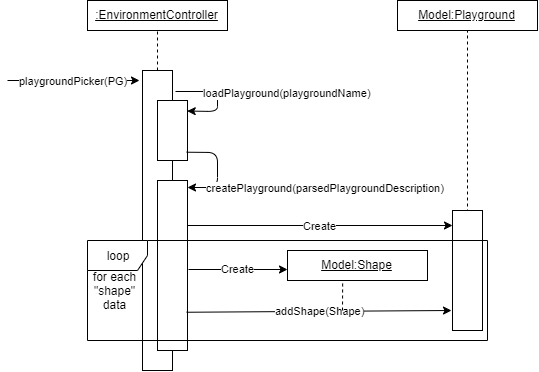
\includegraphics[scale=0.7]{./loadPlayground_sd}
\end{center}

\chapter{Thymio}
\section{What is Thymio} 

Thymio is an educational robot that aims at improving early education (starting in primary school) in Science, Technology, Engineering and Mathematics (STEM),
computational thinking, base computer science and at researching the acknowledgement by kids of robots in their learning environment.
The project also had technical aims, such as how to provide hardware modularity, fast reaction time amid perception and action,
clear internal communication bus in a user-friendly way and streamline development for group robot. This includes direct changes to the robots’ programs and parallel debugging wirelessly, 
transparently and cheaply.\\

The Thymio project is based on a collaboration between the MOBOTS group from the Swiss Federal Institute of Technology in Lausanne (EPFL) and the Lausanne Arts School (ECAL).
MOBOTS being the Miniature Mobile Robots Group, they mainly focus on system design for small robots of the kind. The project started with a strange pile of components, 
that were assembled on any kind of support and hold the name of “Monsieur Patate” (Sir Potato), most likely due to its appearance. 
"Monsieuer Patate" saw life during the first workshop between the two contributors. Afterward, the first “Thymio” was developed, 
it was a four-block robot that could be self-assembled, but not self-programmed as it was delivered with pre-programmed behaviors. 
Thymio was used as a user study to gather feedback from clients in order to know which features needed to be implemented on the Thymio II.\\

\begin{center}
  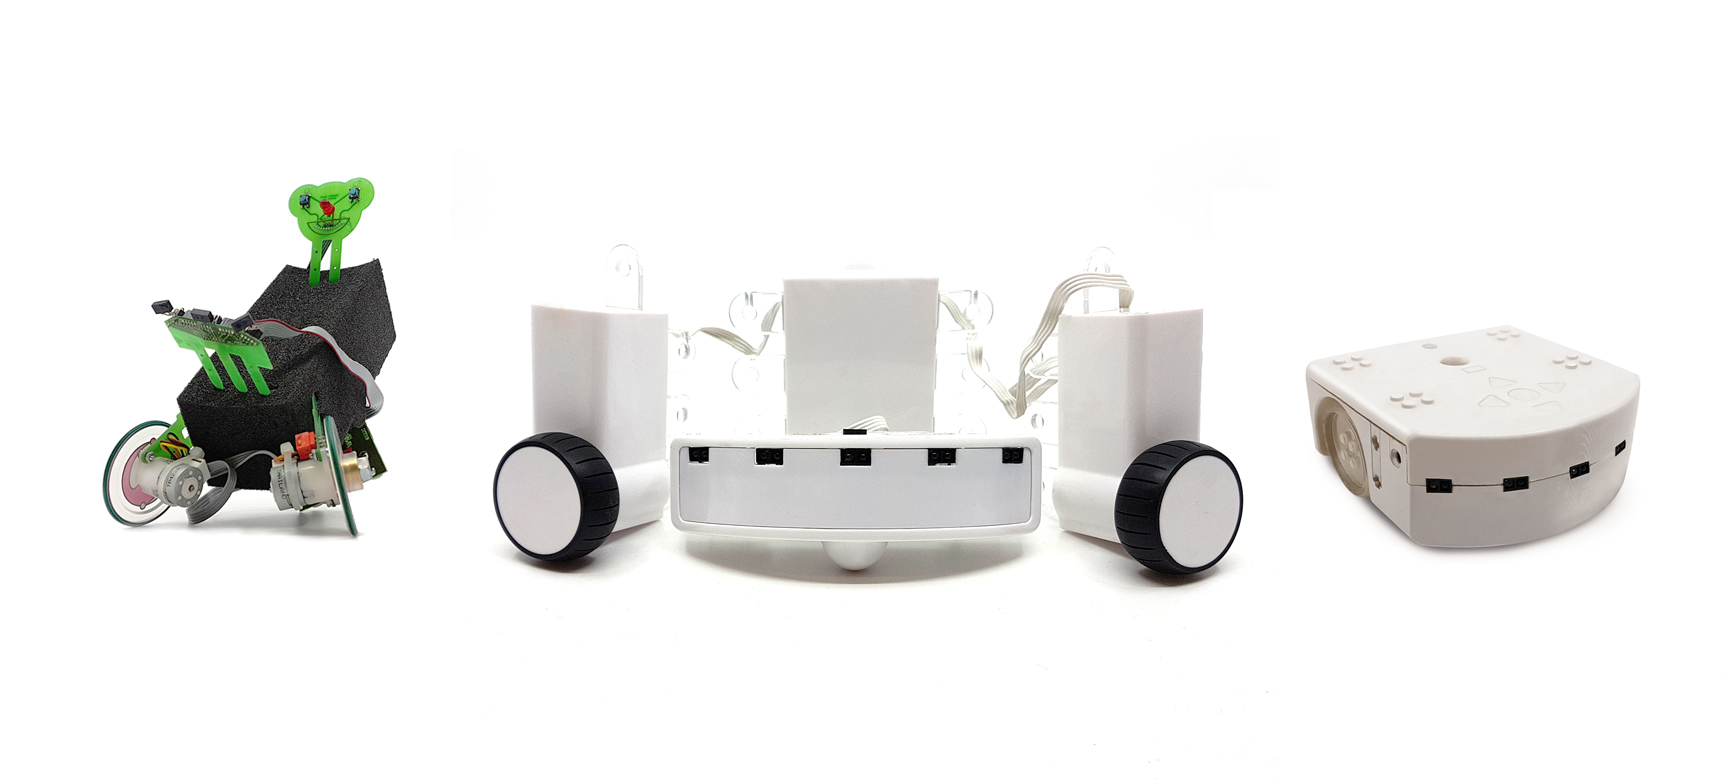
\includegraphics[width=\textwidth]{prototype_thymio_old}\\
  From left to right, "Monsieur Patate", Thymio, Thymio II
\end{center}

The result is a robot with a complex and complete set of sensors and actuators. 
The National Centre for Competence in Research (NCCR) Robotics research program supported the development of the robot. The production distribution and communication of the robot was overseen by Mobsya, 
a non-profit organization that creates robots, software, and educational activities to broaden young people's mind about technology and science. 
Every step of the Thymio project is open-source and has a non-profit aim, namely to enhance the quality of it with the user's project and research as well as to reduce the cost and augment the lifetime for educational platforms and materials.

\begin{center}
  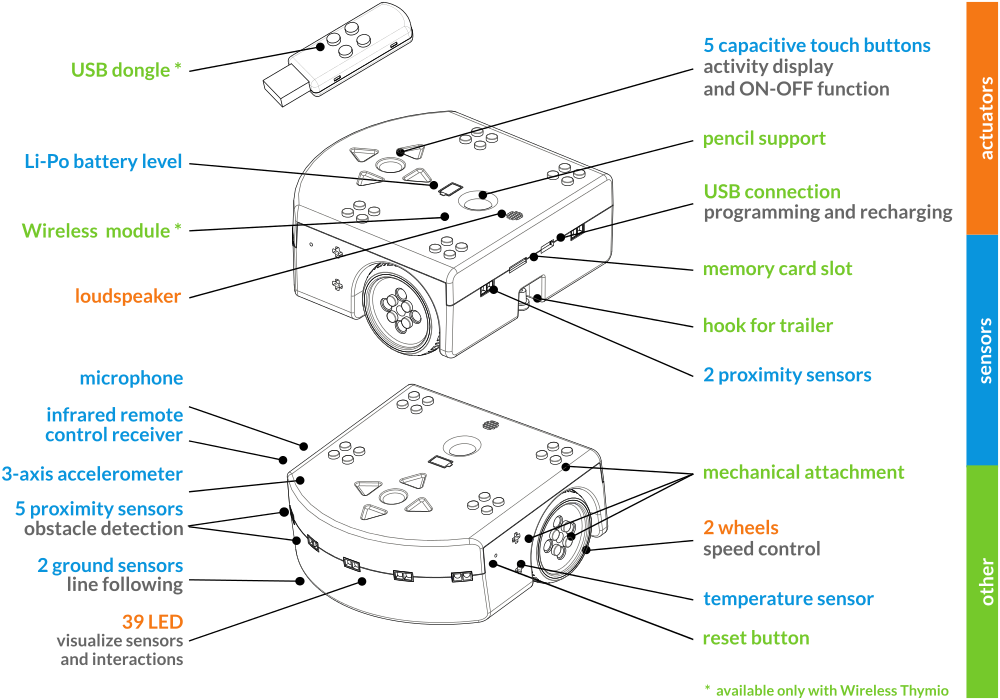
\includegraphics[width=\textwidth]{Wireless-thymioII-sensor-actuator-color-en}\\
  Thymio II sensor and actuator
\end{center}

\section{How does it works \label{howdoesitworkref}} 

As pictured in the figure above there are two Thymio models, namely Thymio and Wireless Thymio. 
The difference between them lies in the ability of the latter one to be programmed wirelessly, 
as suggested by its name. There are two possibilities to begin the creation of a program for the robot there.
The first one, and the most common one for the public is done by using the software Aseba and a connected Thymio. 
In this case, the robot needs to be plugged in via USB cable or USB dongle (possible only if it is the Wireless Thymio) and powered on. 
Then, the software can be used to connect to said robot and to start programming in one of the four different programming languages. 
These are: VPL, Blockly, Aseba, and Scratch. Once the program is ready and sent to the robot it will be available to play. \\

The second option is to use the work-in-progress Thymio Suite version. 
As the software possesses ots pwm bioét-in simulator it does not require a physically or wirelessly connected Thymio robot. 
The same four programming languages are available and one has to be chosen. 
After having selected the language comes the choice of either connecting a physical Thymio or starting a simulation to emulate the programmed behavior.
A more detailed section on the four differents programming languages can be found in section \ref{fourlanguages} on page \pageref{fourlanguages}.

\chapter{Environment}

\section{Three JS}

\texttt{three.js} is a 3D library for \texttt{JavaScript} which uses a default \texttt{WebGL} renderer. It allows the user to display, create and animate 3D computer graphics in a web browser. Its basic rendering pipeline is as follow :

\begin{center}
  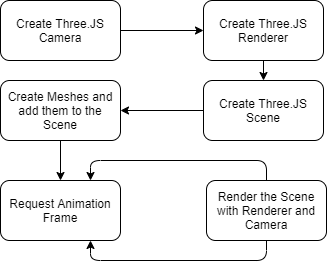
\includegraphics[scale=0.5]{./basic_threejs_rendering}
\end{center}

Every \texttt{three.js} application is composed of at least one \texttt{Camera} element, a \texttt{Renderer} element and a \texttt{Scene} element. The different meshes are added to the scene and this scene along with the camera is rendered using the \texttt{three.js} method 
\texttt{requestAnimationFrame} on the renderer element. 
Using the \texttt{three.js} library it is possible as well to create Augmented Reality application working in web browser. For example it can display information from a database based on a marker. Interesting reading on this topic is available in 
the presentation, examples and discussion of \href{http://jeromeetienne.github.io/slides/augmentedrealitywiththreejs/}{Jerome Etienne}.

\chapter{Architecture \label{Architecture}}

It was decided to divide the architecture into two different parts: one for the simulation side and the other one for the customization. Although they are very similar, there are still some differences that push us to look at them from two different angles. 
Both parts are build based on a \texttt{Model} \texttt{View} \texttt{Controller} system where the elements of the playground, be it a wall or the Thymio robot, are models and the page seen by the user is the \texttt{View}. This \texttt{View} registers the user inputs and transmits them to the \texttt{Controller}. 

As said we have split the architecture, bellow is a graphic representing the architecture for the simulator. The \texttt{Model} \texttt{View} \texttt{Controller} can be seen as well as a second component which is the interpreter. 
The interpreter, is singular to the simulator page. Its role is to test the integrity of the file given as input through the \texttt{Controller} and to compile it into \texttt{JavaScript} code for it to be used as behavior code for the Thymio model.

\begin{center}
  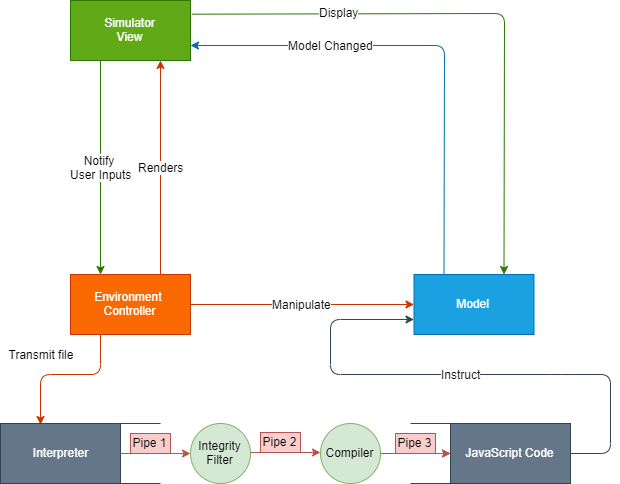
\includegraphics[width=\textwidth]{./architecture_proposal-Page-1}
\end{center}

The used \texttt{MVC} is based on an example from \href{https://github.com/lucasmajerowicz/threejs-mvc-example}{Lucas Majerowicz}. Once the application starts, the following process is run in order to create the \texttt{View}, \texttt{Model}, and \texttt{Controller}.

\begin{center}
  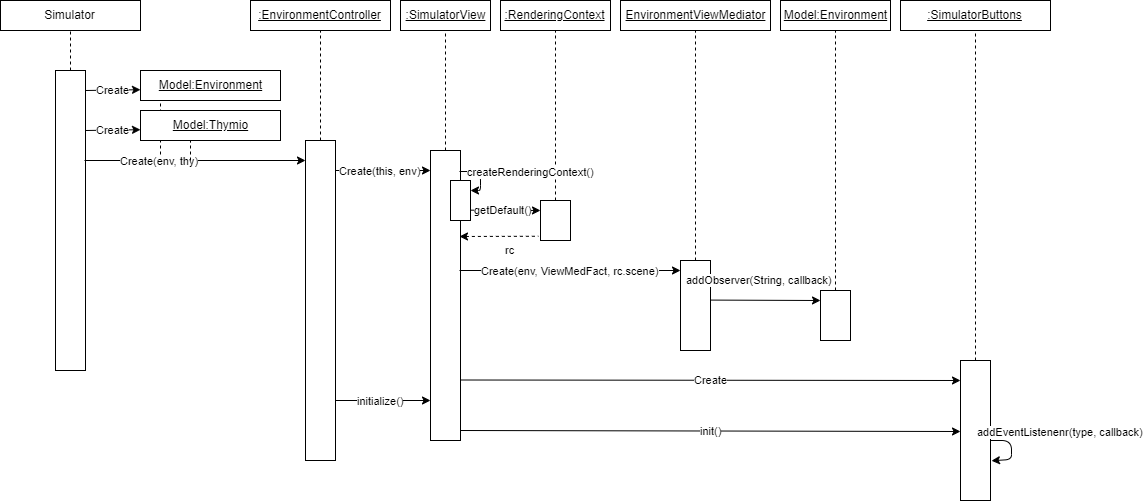
\includegraphics[width=\textwidth]{./start_app}
\end{center}

The \texttt{Model} part is split into three categories. They extends the same base class \texttt{Observable} which works as an event system with the \texttt{addObserver} and \texttt{emit} method. 
The first category is the one responsible for the buttons. We instantiate one of the right types, depending on the \texttt{View}, at the start of the page and add \texttt{addEventListener} to the corresponding \texttt{HTML} elements. 
Those events will trigger the \texttt{emit} method of its base class to notify the \texttt{View} that this particular button has been clicked. The \texttt{View} will catch this event because of the second base method of the \texttt{Observable} class, 
forwarding it to the \texttt{EnvironmentController} class to take care of the logic. 
The two categories left are linked as they operate as the two sides of a coin. They are used for the \texttt{three.js} elements. The first one, the \texttt{Model}, holds the data of the object such as its name, a list of properties containing the dimension, 
color and other attributes for the object. It is those models that are added to the playground element, and whenever a shape is added to the playground, this one will call its base method \texttt{emit} in order to notify the \texttt{ViewMediator}. 
The \texttt{ViewMediator} is the last category and it is responsible for creating the 3D objects with the data from its model. Further, it is responsible for the logic that could be applied to a model, such as the animation of the 3D object, and the supervising of deleting or adding models.     
The image below shows a class diagram of the \texttt{Model} part of the \texttt{MVC}. For clarity purpose, not all classes are represented as their configuration is very similar to one comprised in the diagram.

\begin{center}
  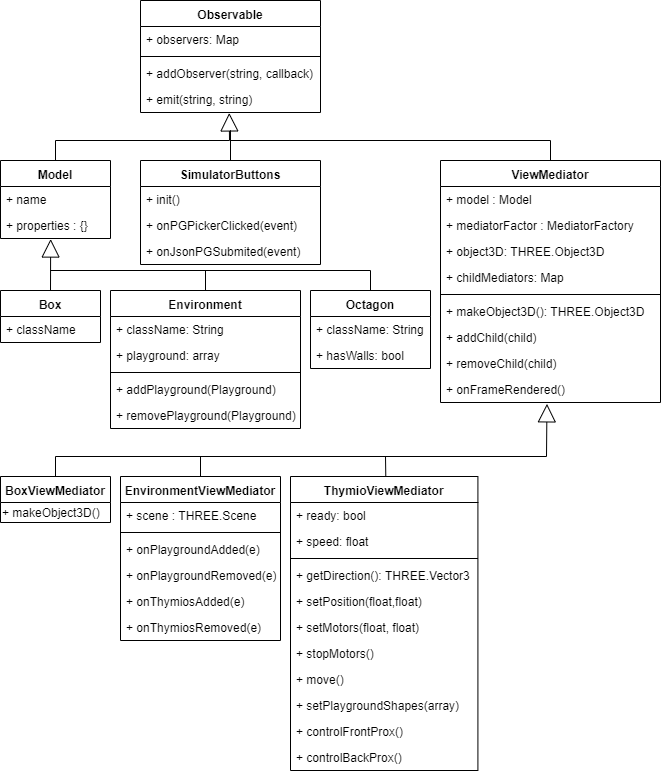
\includegraphics[width=\textwidth]{./mvc_cd}
\end{center}

While the \texttt{View} and the \texttt{Controller} elements are different in the two pages, the \texttt{Model} is not. Int the simulation side, the \texttt{Controller} loads the playgrounds, be it built-in or coming from the device, and uploads the aesl file to the beginning of the filter/compiler. 
In the customization side, it is responsible for writing the \texttt{JSON} file with the data from the meshes of the scene,  instantiating the meshes and registering them once positioned, or deleting them. The two \texttt{Views} are very similar. 
The differences are the observers added to its \texttt{CreatorButtons/SimulatorButtons}, which is how an observer is added.

\begin{lstlisting}[language=JavaScript, gobble=2, basicstyle=\ttfamily\small]
  this.simulatorButtons.addObserver('jsonPGSubmited',
   (e) => this.controller.onJsonPGSubmited(e));
\end{lstlisting} 

Here is the second \texttt{Model} \texttt{View} \texttt{Controller} responsible for the playground customization. Its architecture is the same as the other one, except that it does not implement an interpreter. 

\begin{center}
  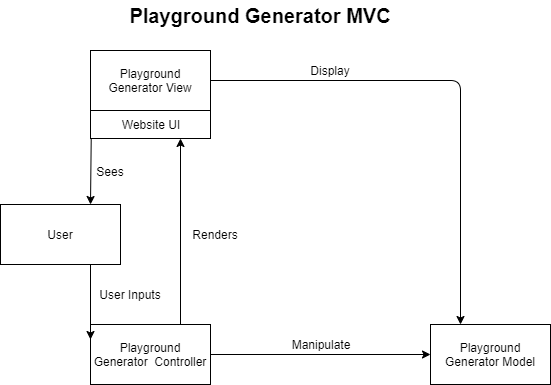
\includegraphics[width=\textwidth]{./architecture_proposal-Page-2}
\end{center}

\chapter{What already exists} 

There exist two possibilities to simulate the behavior of a Thymio II Robot on a computer. 
The first one is through the Thymio Suite application developed by the creator of Thymio. 
It is an application that groups multiple features such as coding the robot in one of the four available languages, 
uploading the program to a real robot or simulating its behavior via a simulator developed in the programming language C++. 
This simulator allows one to load a playground among multiple pre-sets and to run the coded program for the robot.

\begin{center}
  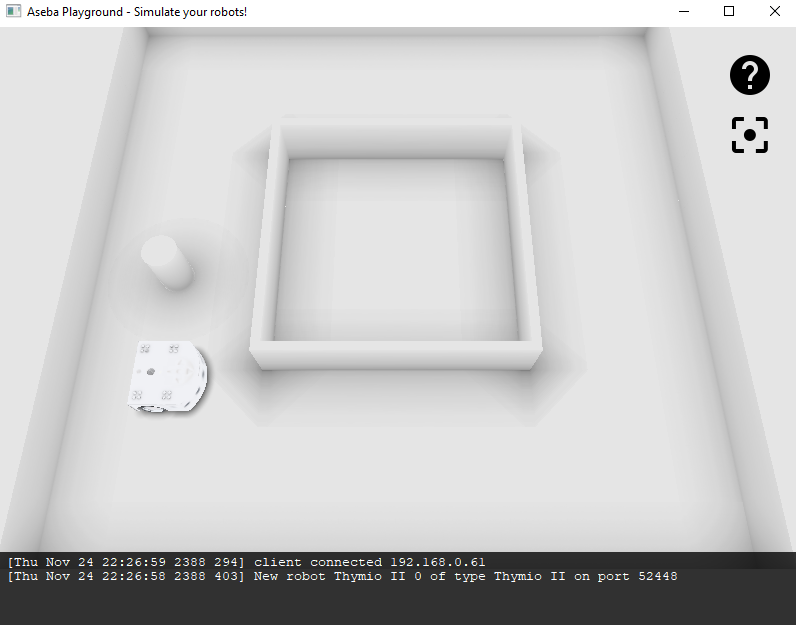
\includegraphics[width=\textwidth]{./suite_simulator}
\end{center}

The second possibility is to use WeBots, which is an open-source 3D robot simulator for industry, education and research purpose. 
It was developed in 1996 at the Swiss Federal Institute of Technology in Lausanne. In 1998 it became a property license software of Cyberbotics, 
and in December 2018 it was lastly released under the free and open-source Apache 2 license.
WeBots is a very powerful software that can do a lot of things. One of these features is an accurate Thymio II model with almost all its sensors and actuator. 
The two Aseba Studio and VPL for Thymio can be directly connected to the software and its simulated robot. 
The specification and usage can be found on their website with the following link \href{https://www.cyberbotics.com/doc/guide/thymio2#mosybas-thymio-ii}{WeBots Thymio} .

\chapter{The Approach}

\section{Base Development}

The first step was to learn how to use the \texttt{three.js} library. Thus, the needed code was directly integrated into some .html file. This integration was not very efficient for a big application, but it was acceptable to test the functionalities. 
At that time, some useful methods that would be needed later on were looked for, such as the way to resize the window and its content. Another functionality added at this period was the control of the camera which comes from the OrbitControls.js file and allows the creation of an OrbitControls object. This object enables the user to move the camera, rotate it and zoom with the mouse.
Afterward, a method was implemented to create different \texttt{Shapes} with more ease for a larger application. Then the scripting part was moved outside of the \texttt{HTML} and inside different \texttt{JavaScript} file as it was not convenient to have all the code into one single \texttt{HTML} file.

\section{WebServer \label{webserver}}
Regarding the goal number 5, "Require no software installation", it was decided to use a webserver in order to access the application. At first, the IIS Manager that is built-in with Windows 10 was chosen.  
The \texttt{ISS} configuration followed the steps shown in this tutorial video: \url{https://www.youtube.com/watch?v=rPRLe7QeVHM} .

Then, the port had to be opened in order to access it from within the LAN. This was done as follows:
\begin{enumerate}
  \item Open the windows Firewall, click on Inbound Rules and New Rule. This will open the New Inbound Rule Wizard.
  \item Select the desired type, Port, click next.
  \item Choose TCP and specify the port used, here 80, click next.
  \item Select Allow connection, click next.
  \item Select all three profile options, click next.
  \item Add a Name and a description to this rule, click finish.
\end{enumerate}

\textbf{Additional setup}\\

It was needed to create a web.config file and to add a few file extensions so that the .mtl and .obj would still be able to load. 
Otherwise, an error of the type "Failed to load resource: the server responded with a status of 404 (Not Found)." was encountered. 
The text that needed to be added to the web.config file is the following one: 

\begin{lstlisting}[language=XML, basicstyle=\ttfamily\small, backgroundcolor = \color{lightgray}]
<?xml version="1.0" encoding="UTF-8"?>
  <configuration>
    <system.webServer>
         <staticContent>
           <remove fileExtension=".mtl" />
           <mimeMap fileExtension=".mtl" mimeType="text/plain" />
           <mimeMap fileExtension=".obj" 
              mimeType="application/octet-stream" />
         </staticContent>
    </system.webServer>
</configuration>
\end{lstlisting}

Unfortunately, after having implemented the new \texttt{MVC} architecture for the application, a further issue was encountered where the application was not able to locate some \texttt{JavaScript} file and gave the following error message in the console : 
\texttt{javascript file not found on server, net::ERR\textunderscore ABORTED 404 (Not Found)}.  After a while of debugging and asking questions to specialists, 
it was decided to move away from ISS Manager. The reasons for this decision were the limited knowledge of this software. The time needed to acquire this knowledge was not worth the effort. 
The alternative solution we came up with was to use \texttt{XAMPP}. As the same version of the application could be pushed without any problem and without having to do anything special, it was decided to continue with \texttt{XAMPP}.

\section{Playgrounds}

It was decided to create three different build-in playgrounds for the application: A basic, with four walls and a square plane; A borderless, composed of a track that leads out of the octagon plane; And one with multiple obstacles, walls and a track. 
Each build-in playground would be composed of one \texttt{THREE.Group} element that is filled with different meshes created from the previously implemented method found in the \texttt{GeometricalMeshes.js} file.

In order to enhance the amount of different meshes, an algorithm to create tracks was added. The tracks creation happened in two steps. The first one consisted into computing a simple line between two points. 
Unfortunately, the result was too thin and therefore a better solution was found.
The second iteration for this algorithm takes an array of points, which are of type \texttt{THREE.Vector3} so as to register the three coordinates, and computes
a new Vector3 that holds the resulting vector position of the next point minus the current point. The x and z values of this vector are then used
as the center to position a box object, which represents the track, and are then aligned to this vector.

\begin{lstlisting}[language=JavaScript, gobble=2, basicstyle=\ttfamily\small]
  for (let i = 0; i < points.length-1; i++) {

    const trackWidth = new THREE.Vector3().copy(points[i+1]).sub(points[i]);
    const track = new THREE.Mesh(
      new THREE.BoxGeometry(trackWidth.length(), TrackHeight, TrackDepth),
      material
    )

    track.position.x = points[i].x + trackWidth.x/2;
    track.position.z = points[i].z + trackWidth.z/2;
    track.quaternion.setFromUnitVectors(new THREE.Vector3(1, 0, 0), 
      trackWidth.clone().normalize());
    container.add(track);      
  }
\end{lstlisting} 

It was decided to load the Thymio model only once, as it takes in average 500ms to 1'000ms to load it, and as some issues where the model would not load every time the playground was changed were encountered.
Therefore, its position and rotation are reset whenever the playground is changed. If a position is given in the playground.json data file, the Thymio is moved to the wanted position.

Thinking about the creation of playground, it was decided to change how the playgrounds data were recorded. Instead of having them as \texttt{JavaScript} files, they were all moved into a \texttt{JSON} file. In this way, it would not require more work to load a 
customized playground later on. To do so, a \texttt{JSON} file of a given name was opened, read, and then skimmed through the \texttt{JSON} file. The \texttt{Shapes} were created accordingly of the data. Bellow an example for the boxes.

\begin{lstlisting}[language=JavaScript, gobble=2, basicstyle=\ttfamily\small]
  if (file.boxes) {
    for (const boxRecord of file.boxes) {
        var box = new Box(boxRecord.name, boxRecord.props);
        playground.addShape(box);
    }
  }
\end{lstlisting} 

Unfortunately, it was later found that \texttt{three.js} has a built-in function which translates a \texttt{ThreeJS} Object into a \texttt{JSON} file element, and inversely. However, dthe solution developed is still being use.

\section{Interpreter}

The interpreter found that compile/translate .aesl file into another programming language is the one used in the Thymio Suite application, its source code can be found in the following repository \href{https://github.com/aseba-community/aseba/tree/master/aseba/compiler}{Aseba git}.
Unfortunately, it is a \texttt{C++} one which means that an operation was needed in order to understand it and find a way to either use it and then use a \texttt{C++} to \texttt{JavaScript} interpreter, or translate the compiler from \texttt{C++} to \texttt{JavaScript} by hand.
The decision was taken to translate the already existing one from \texttt{Aseba} and to start with the compiler. After looking at its behavior and recognizing how it was built and separated,
the time came to translate it to \texttt{JavaScript}. First, the translation creates multiple maps of variable, constant and events. These maps need to be rebuilt with each call to the compiler in case the previous ones produced an error.
Afterward comes the tokenization of the source file, which consists in creating \texttt{Tokens} with the position of the element, its type in the environment, and its value if provided. Then this tokenized source is parsed into \texttt{Nodes}, 
which are expanded and type-checked. Once the program is checked, it is emitted as a first bytecode output. This bytecode is then linked, creating the final program.

The following figure displays a sequence diagram of the compilation of a file.

\begin{center}
  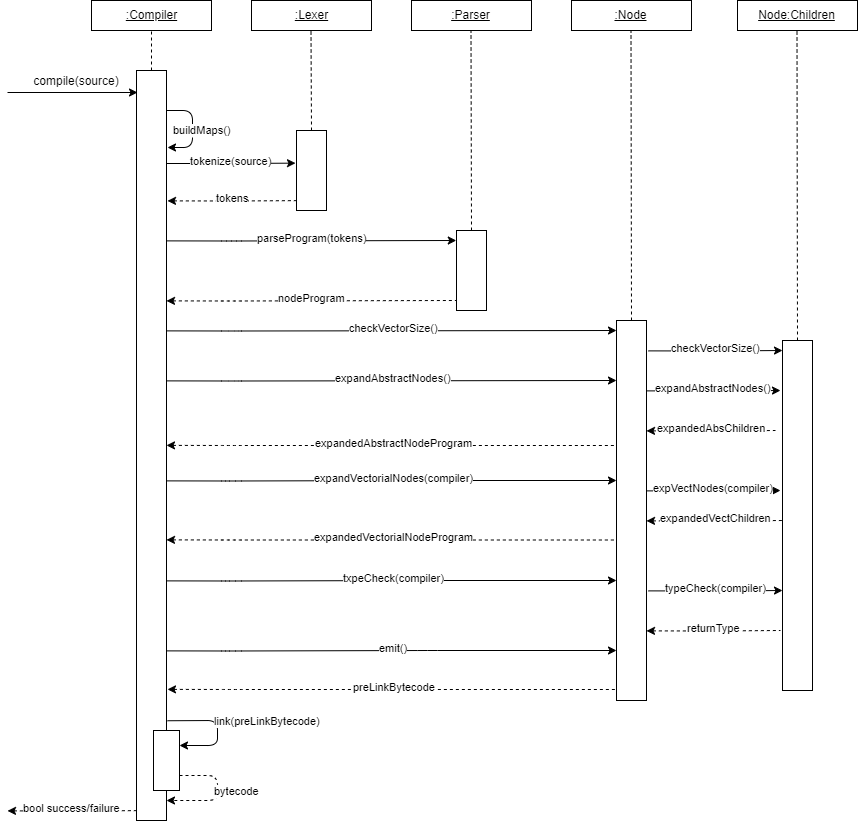
\includegraphics[width=\textwidth]{./compiler_sequence_diagram}
\end{center}

Translating the compiler and everything around was a very hard task for multiple reasons. The first one is the size of the application. Being a large application, it was very hard to understand which component was linked to which, in what manners and how they interacted with each other. A tremendous amount of time was required, scavenging the files and folders in order to try to get an understanding of the architecture.
The second reason is the lack of comments in the source code. Considering the size of the application it was a significant difficulty. In addition to that, it was not planned to work with \texttt{C++} and we were not ready for it. Our knowledge of this programming language is very basic. To summarize, we have a full-scale application coded in a language we are not familiar with and with sparse comments. 
Consequently, it was a very difficult part of the project and could not be completed. 

\subsection{Tokenize}

To tokenize the source file it was needed to skim through the document and switch depending on the value of the character. There are basically five categories for this switch.
The first one comprises the tokens requiring only one character to read, such as \texttt{)} or \texttt{,}. These can directly be given their type. The second category is made of the comments, that is to say the comment block,\texttt{\#* ... *\#}, or the simple line comment,\texttt{\#}. In case of the block comment,
we run through the source in search of the \texttt{*\#} character association that marks the end of the comment block, throwing an error if the character is not found. The third category encompasses the cases that require one character look-ahead.
An example is the character \texttt{+} which could either be a simple \texttt{+} or \texttt{+=} or even \texttt{++}. The fourth is almost the same but with two characters look-ahead, such as \texttt{<}. The fifth category, and the default case of this switch, is the one where the amount of look-ahead needed is not defined.
In this category, the numbers and the strings fit, which are found using a regex as replacement of the \texttt{C++} method \texttt{is\textunderscore utf8\textunderscore alpha\textunderscore num()}. Which controls that the element is either a letter or a number. Below is 
the code for this regex.

\begin{lstlisting}[language=JavaScript, gobble=2, basicstyle=\ttfamily\small]
  isAlphaNumeric(ch) {
    return ch.match(/^[a-z0-9]+$/i) !== null;
  }
\end{lstlisting}

One has to be careful about one point when using this method. If the \texttt{ch} parameter is not a string, then it will throw an error. Coming back to the switch, it first has to be tested if the chain of character is a number. This is done by combining regex and looking for multiple characters.
If the chain of character is not a number, it has to be checked whether its value is the same as the one of the given keywords, such as \texttt{when} or \texttt{const}. In case none of the keywords matches, the chain of character is labeled as a string literal and it is given the value of the chain of characters. Here a problem
of language between \texttt{C++} and \texttt{JavaScript} was encountered, as the type of the token is given with an \texttt{enum} in \texttt{C++} and they do not exist in \texttt{JavaScript}. Consequently, a workaround had to be found in order to solve this language incompatibility. The Object method \texttt{freeze()}, which prevents the modification of existing property attributes and the addition of new ones, 
was used and a value had to be given to each properties.

\begin{lstlisting}[language=JavaScript, gobble=2, basicstyle=\ttfamily\small]
  const type = Object.freeze( 
  {
    TOKEN_END_OF_STREAM : 0,
    TOKEN_STR_when : 1,//"TOKEN_STR_when",
    TOKEN_STR_emit : 2,//"TOKEN_STR_emit",
    ...
  }
\end{lstlisting}

\subsection{Parser}

Once the source file has been tokenized with the Lexer, and no error occurred during the process, the \texttt{Compiler}, that has been partially translated from \texttt{C++} to \texttt{JavaScript}, will pass the tokens as an argument to the parser which will parse it and create a program tree.

The \texttt{Parser} will start by creating a new \texttt{Node.ProgramNode} object with the position of the first element of the tokens array. Then the algorithm will loop on the tokens while it is not empty, and call methods depending on the type of the token. At this stage, the token is split into three categories, namely constant, variable and the rest. 
In the case of constant, the algorithm will check the next token and control that it is of type string. Should this not be the case, the declaration of the constant is not valid and an error is thrown. Should the condition be met, the name of the constant is assigned to a named variable, and the position to a position variable. 
Afterward, the \texttt{Parser} controls that no constant with this name already exists. Then it controls that the next token is of type \texttt{TOKEN\textunderscore ASSIGN} to respect how a constant is declared and gets the value that should be at the next token. If the next token does not belong to the type \texttt{TOKEN\textunderscore INT\textunderscore LITERAL}, it will return the value 0. 
This part will be improved by the completion of the translation of the tree. Finally, the constant with its name, position and value will be added to the \texttt{constantsMap} of the compiler.

If the token is a variable, it will be discarded and the following tokens will be discarded as well if they are part of its declaration. In fact, the part where it would parse the variable was replaced with this removal system. This was done because the \texttt{tree} and the \texttt{parser} are not complete. 
Here is how it should be, if the \texttt{tree} and the \texttt{parser} were finished.

\begin{lstlisting}[language=JavaScript, gobble=2, basicstyle=\ttfamily\small]
  var child = this.parseVarDef();
  if(child)
  {
      programNode.children.addRear(child);
  }
\end{lstlisting}

And this is how it actually is.

\begin{lstlisting}[language=JavaScript, gobble=2, basicstyle=\ttfamily\small]
  this.tokens.removeFront();
  if(this.tokens.front().type === TT.type.TOKEN_STRING_LITERAL)
  {
      this.tokens.removeFront();
      if(this.tokens.front().type === TT.type.TOKEN_STRING_LITERAL ||
         this.tokens.front().type === TT.type.TOKEN_INT_LITERAL)
          this.tokens.removeFront();
  }
\end{lstlisting}

The third part covers the rest of the tokens and is the most complex among the three. The token will go through multiple methods based on a switch on its type until it reaches the parse method that defines it. 
Not every parse method was translated from the \texttt{C++} program as the amount of parse method is rather big and not easy to translate into \texttt{JavaScript}. Below is a diagram showing the process of a token of type \texttt{TOKEN\textunderscore STR\textunderscore onevent} to ease the understanding.

\begin{center}
  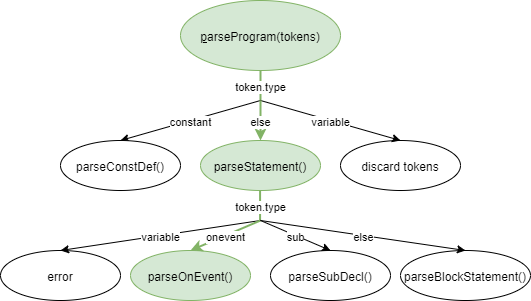
\includegraphics[width=\textwidth]{./event_when}
\end{center}

The end method \texttt{parseOnEvent()} controls two things. First it checks whether an event with this \texttt{Id} exists. Then it verifies that such an event has not been implemented already. The list of \texttt{eventId} can be found in the \texttt{Compiler.js} under the \texttt{buildMaps} method.
If these two conditions are met, a new \texttt{Node.EventDeclNode} with the position and the id of this event will be returned and added to the \texttt{programNode}. 
In case the token is of type \texttt{TOKEN\textunderscore STR\textunderscore when}, the \texttt{Parser} will try to parse the condition and thus will start with the following \texttt{parseOr} method.

\begin{lstlisting}[language=JavaScript, gobble=2, basicstyle=\ttfamily\small]
  parseOr(){
    var node = this.parseAnd();
    while(this.tokens.front().type === TT.type.TOKEN_OP_OR)
    {
      var pos = new SourcePos();
      pos.setValues(this.tokens.front().pos);
      this.tokens.removeFront();
      var subExpression = this.parseAnd();
      var temp = new Node.BinaryArithmeticNode(pos.getValues(), 
        Node.AsebaBinaryOperator.ASEBA_OP_OR, node, subExpression);
      node = temp;
    }
    return node;
  }
\end{lstlisting}

As it can be observed, this method starts by calling another one. This will go on and on until very low methods such as the \texttt{parseUnaryExpression}.

The tree that is built during the parsing which contains the \texttt{programNode}, \texttt{eventNode} and every other node, is created based on the following class diagram.

\begin{center}
  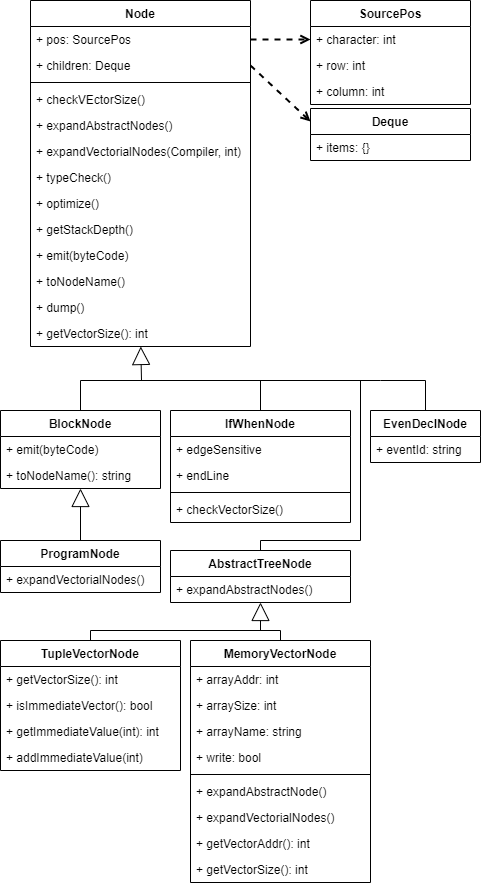
\includegraphics[scale=0.6]{./tree}
\end{center}

This is the point that was reached, for more information on the possible completion and future work refer at the section Future research on page \pageref{future}.

\section{Phyisics}

Adding physics allows collisions between the robot and the different objects. It's been tried to use \texttt{Physijs}, the source code can be found in the following repository \href{https://github.com/chandlerprall/Physijs/wiki/Basic-Setup}{Physijs git}, 
but with the architecture of the application, a problem was encountered due to the fact that \texttt{THREE.Object3D} are added instead of basic mesh and \texttt{Physijs} works only with a fixed amount of meshes. A solution would be not to use \texttt{Physijs} as it is only needed for the \texttt{Thymio} to move and to stop upon collisions.
Instead of \texttt{Physijs}, the robot could shoot rays in order to check for collisions.

\section{Sensor and Actuator}

The five buttons that sit on top of the \texttt{Thymio} were represented directly in the \texttt{UI}. There was no interaction with the modelized ones. Initially, we wanted to create a directional pad style group of buttons similar to the one on the first image below. 
However, due to time constraints, the created group of buttons could not be perfectly arranged, as pictured on the right.

\begin{center}
  \begin{tabular}{c c}
	  1  & 2 \\
    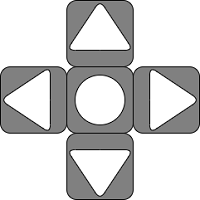
\includegraphics{dpad} & 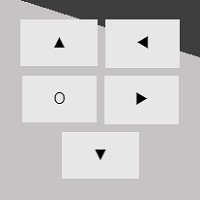
\includegraphics{fake_dpad}
  \end{tabular}
\end{center}

A \texttt{Thymio} robot moves according to two motors, one for its right wheel and one for its left wheel. They have a value for the output power between -500 and 500, where the minus sign means that the motor powers the wheel in the opposite direction. 
Those two motors can only output power in a straight line, forward / backward. Below are displayed three representations of the expected movements of a \texttt{Thymio}. The yellow arrow is the power for the left motor, the blue arrow is the power for the right motor, 
and the green arrow is the final vector movement for the robot. On the first representation, the power of the two motors is the same, both in value and direction. Thus, the final vector is simply the same as either one of the two.
On the second representation, the value of the power for both motors is still the same but their direction is opposite. Hence, the final vector is a circle because the robot will turn on itself.
Finally, the third representation shows the resultant vector when the value is not the same but the direction is.

\begin{center}
  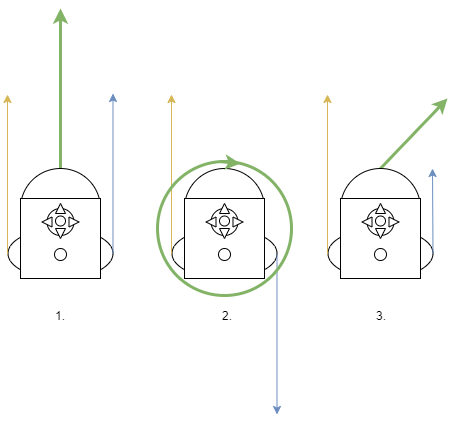
\includegraphics[scale=0.8]{./thymio_move}
\end{center}

It was complex to convey the way the Thymio robots move onto this application as we move models and do not physically power motors. To achieve the same behavior, it was decided to resort to trigonometry and a few tricks.
The method that moves the robot is called only within the \texttt{render()} method from the main View, and thus every time the scene is being rendered, the robot is moved according to the value of the motor. 
Those values are set using the \texttt{setMotors(left, right)} method. The \texttt{move()} method, the one that computes the movement of the robot, is split into four categories depending on the values of the motors. 

The first category is when both motors have the same power in the same direction. Thus, the resulting position change for both x and z coordinate is computed using the \texttt{getDirection()}, which returns 
a Vector3 representing the direction the robot is facing, a predefined speed variable and the power given to either of the motors.

\begin{lstlisting}[language=JavaScript, gobble=2, basicstyle=\ttfamily\small]
  getDirection() {
    var direction = new THREE.Vector3();
    return this.object3D.getWorldDirection(direction);;
  }
\end{lstlisting} 

\begin{lstlisting}[language=JavaScript, gobble=2, basicstyle=\ttfamily\small]
  this.object3D.position.x += 
    this.getDirection().x * this.speed * this.rightMotor;
  this.object3D.position.z +=
    this.getDirection().z * this.speed * this.rightMotor;
\end{lstlisting}  

\begin{center}
  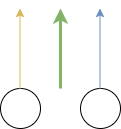
\includegraphics[scale=0.8]{./move_spsd}
\end{center}

The second option is when the value of the left motor is bigger than the one of the right one, regarding the direction. Alternatively, the third option is the same but when the value of the right motor is bigger than the one of the left one.

\begin{center}
  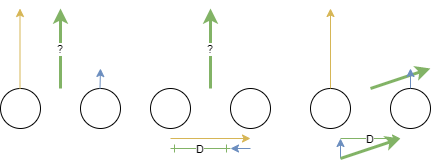
\includegraphics[width=\textwidth]{./move_dp}
\end{center}

In this case, we calculate the difference \texttt{D} of power between the two motors, subtracting the smallest from the biggest. Then, trigonometry was used to find the angle between the power of the motor and the resulting vector of the addition of the power of the motor and the difference \texttt{D}.
This angle is then used as a parameter to rotate the model around the y-axis. In order to smooth the rotation, we multiply it by a variable turnSpeed.  

\begin{lstlisting}[language=JavaScript, gobble=2, basicstyle=\ttfamily\small]
  this.object3D.rotateY(
    -(Math.atan(delta/Math.abs(this.leftMotor))*this.turnSpeed)
  );
\end{lstlisting} 

The resulting change in position is computed the same way as for the first category. It might be more relevant to use the norm of the resulting vector 
found earlier to have a more accurate speed.

The fourth category happens when both power values are the same but in a different direction. In this case, the robot is rotated on itself around the y-axis according to either one of its motor speed.

\begin{center}
  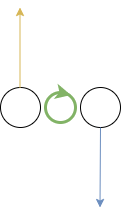
\includegraphics[scale=1]{./move_spdd}
\end{center}

However, this algorithm has a few flaws. One of these happens when the power of one motor is 0. While the robot should be rotating on itself with the said motor as an anchor point, it rotates and moves in the direction of the second motor's direction.


In order to determine whether a collision occurs between the robot and one of the elements of the environment, it was decided not to use an external physic library but rather to throw raycast from various positions in the thymio model. In this sense, we instantiated a \texttt{THREE.Raycaster} 
object and looked for a way to get all 3D objects from our scene. This was quite troublesome because of the implementation of our model view controller. When instantiating a new \texttt{Model} we would not get a reference to its \texttt{ViewMediator} where the model is stored. 
We used the benefit of \texttt{JavaScript} to find a workaround Whenever a \texttt{ViewMediator} is instantiated, the property \texttt{mediator} is added to its model where the value is the current mediator. Thus, the method displayed below was used in order to skim through the array containing the shapes rendered in the scene and create a new array filled with intersection objects. Then, the array was loop through to control that the distance is bigger than the given one. If not it operates an action depending on the \texttt{className} of the intersected object. 
In the default case, we assume that the robot encounters an element against which he should stop moving.

\begin{lstlisting}[language=JavaScript, gobble=2, basicstyle=\ttfamily\small]
  intersects = raycaster.intersectObjects(this.shapes, true);
  for(let i = 0; i < intersects.length; i++){
    if (intersects[i].distance < 3.5){
      if(intersects[i].object.mediator.
          model.className === "Plane" ||
         intersects[i].object.mediator.
          model.className === "Octagon"){}
      else if (intersects[i].object.mediator.
          model.className === "Track"){}
      else{
        this.stopMotors();
      }
    }
  }
\end{lstlisting} 

A variant of this algorithm was used in order to control the ground collision. Thus allowing the robot to know if it is progressing on the ground or not. If the robot is not progressing on the ground, the algorithm would make it fall by changing its \texttt{Y} coordinate.
However, for some reasons the \texttt{intersectObjects} method would not detect any intersection if the robot was in the upper half part of the playground. Thus, the ground check were disabled.

\section{Customize playgrounds}

The creation of a customize playground that can be used later on in the simulation part of the application takes place on a different page. On this page, the architecture is the same as for the simulation, but the \texttt{Controller} as well as the \texttt{View} elements are changed
and the compilation part is excluded. Thus, most of the changes and logic come from the \texttt{CreatorController.js} file. We reflected on how the data of the playground would be carried, or kept, and used in the simulator. Thus, multiple options appear,
such as using a database to store every customed playground so that they would all be available with the application. Another option would be to download them locally as a file on the user's computer. We continued with the latest option as we previously prepared the program to load playgrounds from \texttt{JSON} files.
Saving the playground data is done in four different steps. A sequence diagram of the process is shown below.

\begin{center}
  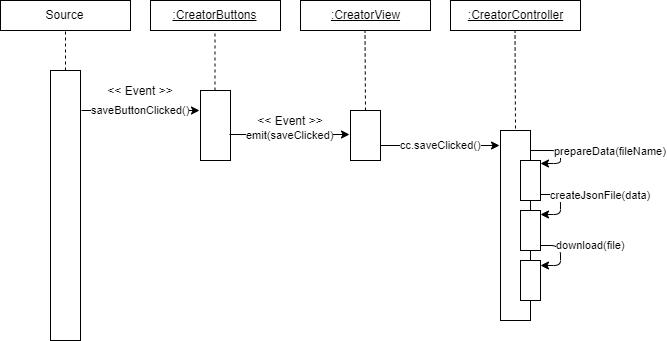
\includegraphics[scale=0.55]{./savepg_sd}
\end{center}

First, once the event that the \texttt{saveButton} has been pressed is thrown, the application will open a \texttt{prompt} window in which the user will specify the file name. Then, the data that composed the customized playground are being separated into different arrays based on their \texttt{className} property. 
Once the shapes contained in the customized playground have been gone through and categorized, the final \texttt{JSON} file is created. Its creation uses the \texttt{forEach} method of \texttt{JavaScript} array and writes the name of the mesh as well as its properties. 
Finally, the file is downloaded on the user's computer and the process ends. The \texttt{JSON} file obtained looks like as follow.
%% TODO : Be sure it is not in between two pages

\begin{lstlisting}[language=json, basicstyle=\ttfamily\small]
  "playground":"jailtype",
    "octagons":[
        {
        "name":"ground",
        "props":{
            "segmentLength":35.5,
            "color":"#bdbbbb"
            },
        "hasWalls":true
        }
    ],
    "boxes":[
        {
        "name":"Box0.5",
        "props":{
            "width":4,
            "height":10,
            "depth":21,
            "color":"#ff0202",
            "positionX":0.5,
            "positionZ":-17.5,
            "rotateY":1.6755160819145565
            }
        },
\end{lstlisting}

It was needed to add a few more controls over the scene in order to increase the ease of use and the possibilities of creation. The camera controls need to be enabled so that the user can navigate through the scene but once the user chooses his desired location for
the mesh, he needs to deactivate those controls with the \texttt{shift} key, and enabled them back with the same key. It was decided to add three other controls. The first is the use of the \texttt{Esc} key to cancel the current mesh positioning. This control removes the current placeholder from the scene. 
The second and third are linked with each other. It is the use of the \texttt{ctrl-Z} and \texttt{ctrl-Y} logic. To do so we create two different arrays, one with the current meshes in the scene and the other one with the removed meshes, which operate as \texttt{LIFO} Queue.
However, we test that the length of the respective array is legal to perform the action and that the current shape being created by the user is from the type \texttt{Tracks}. Then, another logic is applied, which removes/reinserts the last point of the track.
There are three different shapes at the user's disposal and two types of grounds. A ground element will always be needed to save the current playground, otherwise, an error occurs. The two types of grounds are a simple rectangle and an octagon, with a set of properties. 
Changing the properties will not change the mesh in real-time, but once the button \texttt{Generate Ground} is pressed it will remove the previous ground and add the new one. The creation of boxes and cylinders takes part in two steps. 
During the first step, the user will choose the properties, such as the \texttt{width}, the \texttt{length}, the \texttt{height}, the \texttt{color} and the \texttt{rotation} for the box. Then, by clicking the \texttt{Generate} button of the shape, 
a placeholder of the shape will be instantiated and it will follow the movements of the mouse while rounding its position to fit into the square represented by the \texttt{THREE.GridHelper} element. 

\begin{lstlisting}[language=JavaScript, gobble=2, basicstyle=\ttfamily\small]
  this.rollOverMesh.position.divideScalar( 1 ).floor()
    .multiplyScalar( 1)
    .addScalar( 0.5 );
\end{lstlisting} 

Afterward, the user has multiple-choices. He can either click to fix the mesh onto the scene, or the properties did not fit what he wanted so he would click once more on the \texttt{Generate} button with the new properties, 
or cancel the action with the \texttt{Esc} key. 
In order to lay Tracks, it was needed to create one more step as the mesh is composed of multiple points. Those points are laid the same way as a \texttt{Box} mesh would be but they are added to an array that stores the position of those point. 
Once the track is finished and upon clicking on the \texttt{Generate Track} button the points placeholders will be removed and a track passing through the wanted positions will be computed by looping through the points array and feeding the property element of track with the position of \texttt{X} and \texttt{Z} of each points. 
It was necessary to delete the last point added as it was registering and instantiating a point when the user was clicking on \texttt{Generate Track}.

\begin{lstlisting}[language=JavaScript, gobble=2, basicstyle=\ttfamily\small]
  this.points.forEach(pt => {                      
    this.props.points.push({
      positionX : pt.position.x,
      positionZ : pt.position.z
    });
  });
\end{lstlisting} 

However, the algorithm tracking the movement of the mouse and changing the position of the temporary mesh is not optimized and will slow down the application drastically. Unfortunately, we do not know which part of the algorithm has to be optimized.

\section{Incorporated Behavior}

The \texttt{Thymio} robot has multiple pre-programmed behavior which can be chosen using the central button of the D-pad. Thus, three behavior were implemented in the simulation as well. First, a basic behavior. This behavior allows user to input power to the motors using the D-pad.
Second, is an explorer behavior. In this state, the robot will act as an explorer by moving forward and upon collision with an element of the playground, it will drive back, turn and drive forward again until it is stopped by the user.
To achieve this sequence of instructions, a \texttt{JavaScipt} method that allows a delayed call to a function was used. It is the \texttt{setTimeout} method, which was used to stop the motors after a given time and start to turn.

\begin{lstlisting}[language=JavaScript, gobble=2, basicstyle=\ttfamily\small]
  this.setMotors(-250,-250);
  var thm = this;
  this.timeOuts.push(setTimeout(function(){
    thm.stopMotors();
    thm.halfTurn(true);
  },1000));
\end{lstlisting} 

The third behavior that was programmed, is a track follower one. Upon pressing the forward button, the robot will look for the closest point of the track and start to follow the track from that point.
It was decided to reach the points from the track starting by the closest one, so the previous would be discarded. Although by uncommenting a line in the code this behavior can be achieved.

\begin{lstlisting}[language=JavaScript, gobble=2, basicstyle=\ttfamily\small]
  var smallest = 100;
  var index;
  for (let i = 0; i < this.points.length; i++) {
    if (this.object3D.position.distanceTo(this.points[i]) < smallest)
    {
      smallest = this.object3D.position.distanceTo(this.points[i]);
      index = i;
    }            
  }
\end{lstlisting}

In order to reach the next point the algorithm is not using the motors of the robots, this could be improved. To control whether the robot is close enough to the target point a method is called, in the \texttt{onFrameRendered} method only if the state corresponds to the track follower,
and if the robot is following a track, which will change the behavior depending on the distance to the target and the number of points left.

\chapter{Conclusion}

\section{Results}

We have reached five out of the six goals that were determined at the beginning of the project. We have created an environment where a \texttt{Thymio} robot can move around a given playground. The playground can be chosen between built-in ones and others that are fully created by the user with a tool enabling it.
One sensor and three actuators have been analyzed and implemented into the robot, the proximity sensors, the two motors, the lights, and the top d-pad buttons. We have also noticed that although our application architecture, \texttt{MVC}, allows the addition of new models very easily, it is too heavy and restrictive in terms of diversity. 
For example, to add the proximity sensors we had to implement them in a non-optimized manner. The application runs smoothly, except for the placement of new meshes in the playground creator due to an algorithm issue, 
on any modern browser without further installation required and is accessible from inside the \texttt{BFH} network. Unfortunately, it is not possible to input a .aesl file containing a program to the application and to use it as a behavior for \texttt{Thymio}. 
Thus, the sixth objective, the \texttt{Integration of Aseba Language}, was not brought to terms due to multiple problems and issues. As we came into this project without experience regarding the creation of a compiler/interpreter, we underestimated greatly the amount of work required by this part during the project. 
We decided to use an already existing compiler/interpreter, namely the one from Aseba used for their \texttt{Thymio Suite} application. The code was written in \texttt{C++} and considering our basic knowledge of this programming language, it was a second slowdown in the project.
Thus, it was rather difficult to convert this program into JavaScript. However, in order to compensate for this, we analyzed a \texttt{Thymio} robot and discovered that it is delivered with some built-in behaviors. Consequently, we decided to incorporate two of them to demonstrate that a web simulation of a \texttt{Thymio} is possible. 
In addition to that, if the steps in the next section are brought to completion it is completely possible to fulfill the integration of the \texttt{Aseba} language into the application.

\section{Future research \label{future}}

In order to continue this project the next step would be to complete the goal that could not be brought to an end. This would require to finish translating the various \texttt{.cpp} and \texttt{.h} file from the folder compiler of \href{ https://github.com/aseba-community/aseba/tree/master/aseba/compiler}{Asebas Git}. 
The further step of the process of compiling a file would be to implement the \texttt{checkVectorSize} method. This method recursively walks through the tree and checks the different \texttt{Nodes} vector size and throws an error in case the return value does not match the expected one. 
The \texttt{compiler} would then continue on to expand the syntax tree to \texttt{Aseba} like syntax, through a recursive walk on the tree. The tree would be recreated with the new syntax. Afterward, it would expand the vectorial nodes into scalar operations and rebuild the tree. 
In the next step, the type of each node would be checked to see if it corresponds to the expected one. It would then optimize the current tree, and then emit the first \texttt{Bytecode} generated from the tree. 
Using a subroutine table, the compiler would fix-up the generated \texttt{Bytecode} that might be missing some \texttt{STOP} or \texttt{RET}. Then, the \texttt{verifyStackCalls} method, as its name suggests it, would verify the integrity of the stack with no overflow. 
And it would end by linking the bytecode into the final program. Here, the linking is a flattening of complex structure into linear vector.

Once this part would be over, more sensors could be added. Those sensors could, for example, be sound sensors to listen to the clap of hands, or a "Pen holder" to draw figures by moving Thymio around. 
Ideally, a way to ease the addition of sensors and actuators would be designed and implemented. It could be something similar to our \texttt{Model} / \texttt{ViewMediator}. And to improve the already existing one. For example by getting rid of the algorithm issue on the motor actuators.

\section{Personal conclusion}

The work on this thesis was very interesting and challenging. There were many new technologies to learn, understand and master. Initially, we did not expect to be confronted with a full-scale \texttt{C++} application, but we have learned a lot from it.
The difficulties that emerge when translating a program in one programming language into another programming language were also very instructive. We observed that it was rather difficult to estimate the amount of work needed for the various part that we were not accustomed to.
For example, the compiler was very time-consuming, while the customizable playground required less time. In conclusion, we gained a lot of knowledge and experience during this project.


\appendix

\chapter{The different programming languages \label{fourlanguages}} 
\section{VPL}

One of the four different possibilities to program the Thymio is by using the visual programming language, or VPL, 
developed by the creator of Aseba. A visual programming language is an abstraction of the more common way to program. 
It is based on the manipulation of program elements graphically that can be manipulated following some spatial grammar to create a program. 
VPLs are based on a set of entities and relations, whereas most of the time entities are represented by boxes, 
or other graphical objects, and relations by simple arrows. They can be categorized into icon-based, 
form-based and diagram-based languages depending on the extent of visual expression inside of them. 
The use of visual programming languages can be found in multiple areas, such as the game engine “Unreal Engine 4” where their system of Blueprints is created upon a node-based VPL, 
or “Microsoft SQL Server Integration Services”. This abstraction allows easier access for neophytes, 
for example using graphic elements such as blocks, forms, diagrams, and others which reduce drastically, if not eliminate, the syntactic errors made by the user.\\

In the case of the VPL developed by Aseba’s team, the one we are mostly interested in, it is a programming language based on two types of blocks: Event blocks and Action blocks. 
Based on those two blocks, the seventeen, respectively eleven event blocks and six action blocks, entities are built. 
One of the main goals of VPL for Thymio was to enable people who cannot yet read to start programming and discover this world.\\

\begin{center}
  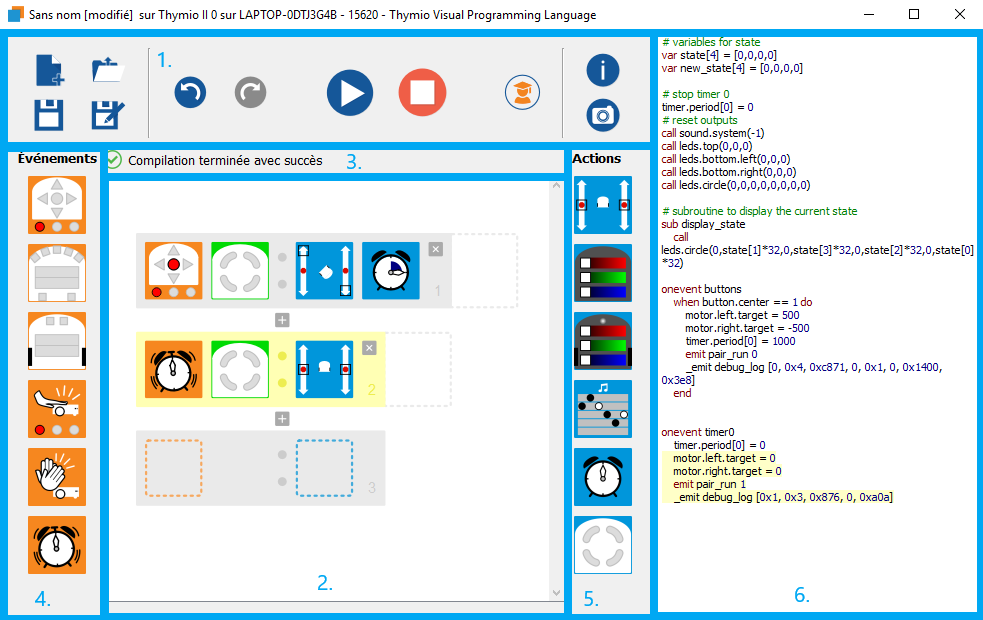
\includegraphics[width=\textwidth]{./VPL/Thymio_VPL_window}\\
  Thymio VPL Event and Action blocks
\end{center}

To begin creating a program follow the first steps described in section \ref{howdoesitworkref} on \pageref{howdoesitworkref}. 
Once the VPL option has been chosen and the Thymio Visual Programming Language window appears programming begins. 
The window is split into six different regions, where each has its own purpose as listed below.
\begin{enumerate}
  \item A tool bar
  \item A programming window
  \item Console messages
  \item The event blocks
  \item The action blocks
  \item The program translated into AESL
\end{enumerate}

\begin{center}
  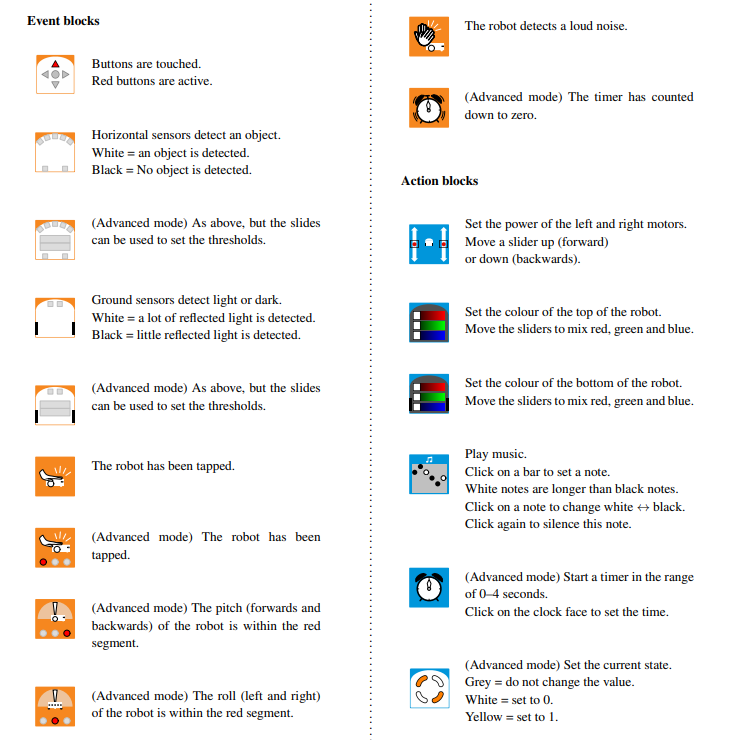
\includegraphics[width=\textwidth]{./VPL/Thymio_blocks}
  Thymio VPL Window
\end{center}

At first, the programming window is empty of blocks, containing just a placeholder with empty slots. 
This placeholder is the base of every Thymio VPL program. It contains exactly one event block and one or more action block. 
This means that whenever the event of the event block happens, then the set of actions added to this placeholder will occur at the same time. 
For example, with the following pair: \\
\begin{center}
  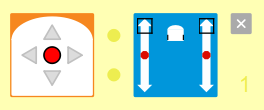
\includegraphics[scale=0.5]{./VPL/middlebtn_forward}\\
  Event and one Action relation
\end{center}

Both wheels are powered to the maximum when the middle button is pressed. However, more than one action can be attributed to one event. 
In order to do that, another action block has to be dragged into the previous pair. It should be noted that the same block cannot be used twice for the same event. 
Here we turned the lights on top and set them to a complete green:\\
\begin{center}
  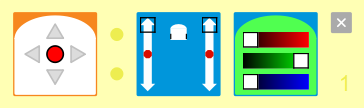
\includegraphics[scale=0.5]{./VPL/middlebtn_forward_green}\\
  Event and multiple Actions relation
\end{center}

The maximum amount of action blocks we can add to an event is four, but we can add as many event blocks to our program as we want. 
Let us add two more event blocks to allow the robot to turn:\\
\begin{center}
  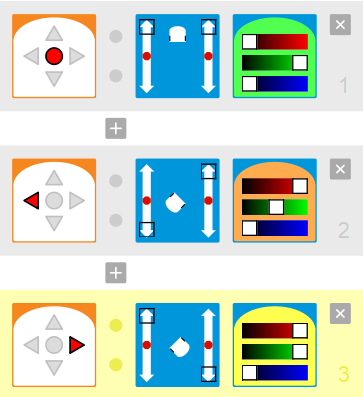
\includegraphics[scale=0.5]{./VPL/middlebtn_3E}\\
  Event and Actions relations
\end{center}

Now we have a basic behavior: go straight with green lights when the middle button is pushed, turn left on itself with orange lights when the left button is pushed, 
and at last turn right on itself with yellow lights when the right button is pushed.\\

By clicking the button with a student as an icon we enable the advanced mode that gives us more possibilities for multiple blocks. It raises the amount of action block from four to six as well. \\

Let us refactor a bit the program from before. We will change the program by making the robot look left then right and starting over again using timers. 
In order to help us develop a more interesting program, we have now access to a condition, namely a four led light on top of the robot. Using this and the timer we can behave depending on the state of the robot. 
For example, hereafter the middle button was pressed a timer will start and after a short amount of time, it will light one particular led. 
Afterward, the event “timer elapsed” will be triggered. However, it has to be decided which pair should be executed by the program, namely turning right or turning left? 
Hence comes the use of the condition as we will execute the part of the program that corresponds to the state of the condition light. 
In this example, it will go back and forth between the two pairs: \\
\begin{center}
  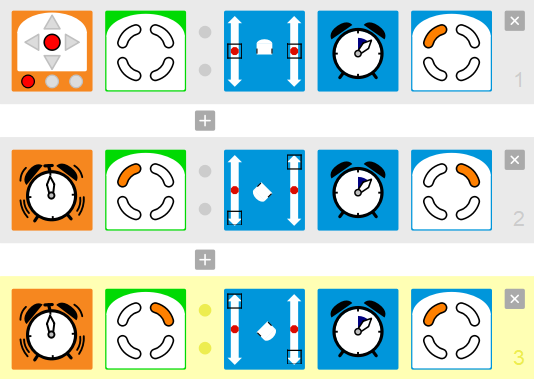
\includegraphics[scale=0.5]{./VPL/middlebtn_3E_adv}\\
  Advanced program
\end{center}

\section{Blockly 4 Thymio}

The second possibility to program the \texttt{Thymio} is to use \texttt{Blockly4Thymio}, which is an environment based on Blockly. Blockly was released in May 2012 and was initially a replacement for OpenBlocks for the \texttt{MIT App Inventor}. 
It is an open-source client-side library that allows its users to easily add a block-based visual programming language to an application or website. 
Blockly is not in itself a programming language but it is rather used to create one. Its design makes it flexible and it can support a large set of features. 
As it is a visual programming language, it shows similar advantages to the first possibility. For example, it can apply programming principles with no regard towards syntactic error.
Blockly is among the growing and most used visual programming environments because of a few important features. First, it can export the code generated with the blocks to one of the five following programming languages, 
as a built-in feature, \texttt{JavaScript}, \texttt{Lua}, \texttt{Dart}, \texttt{Python}, and \texttt{PHP}. Second, it can be enhanced for any textual programming languages. 
The block pool can be expanded from its base pool or even reduced depending on the needs. The blocks are not restrained to only basic tasks and can implement sophisticated programming tasks. 
Additionally, it has been translated into over forty languages, and there exist right-to-left versions. \\

Blockly includes a set of pre-defined blocks that can be used to develop more easily the wanted application. They are arranged into eight families:
\begin{description}
  \item [Logic:] Blocks with Boolean definition, equality check, and conditions.
  \item [Loop:] Blocks for loops.
  \item [Math:] Blocks for numbers, arithmetic operations, a few basic math functions (for example cos, sin, square root) and some mathematical constant (Pi).
  \item [Text:] Blocks to create text and text operations.
  \item [Lists:] Blocks to create lists and standard list operations (length, get the value).
  \item [Color:] Blocks with a color definition.
  \item [Variables:] Blocks to create variables, and to set/get their values.
  \item [Functions:] Blocks to create functions, with return value or not, and to call existing function.
\end{description}

Each block holds a pre-assigned shape, thus restraining its usage to certain situations as a "hidden" way to control the syntax. Their shapes are defined by the different connections with other blocks, 
both external and internal. While external blocks describe what happens after or before, the internals ones describe what happens during or what are the arguments, the logic. 
Following is a basic variable block with three external connectors, and a math block with the value of one, with one connector, that is assigned to the \texttt{Count} variable (the blocks need to be assembled). \\
\begin{center}
  
\includegraphics[scale=0.5]{./Blockly/basic_variable}\\
  Variable block
\end{center}

Using the same logic as above we created a \texttt{Limit} variable with the value of 5 to demonstrate the next example. 
The block used is from the logic family and it tests whether the \texttt{Count} variable is smaller or equal to the \texttt{Limit} as internal blocks. 
It can then be added to a loop, a function or to other statements that needs logic.\\
\begin{center}
  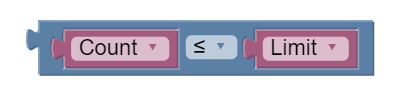
\includegraphics[scale=0.5]{./Blockly/basic_logic}\\
  Logic block
\end{center}

Added to the base that Blockly is for \texttt{Blockly4Thymio}, is a compilator that interpret and adapt the Blockly code directly into Aseba language, and an Aseba Framework. 
Let us once again follow the steps described in the “How does it works” section in order to start blockly-ing a small program with \texttt{Blockly4Thymio}. 
Note that it is possible to open the \texttt{Thymio Blockly} environment without going through the Thymio suite, and without any Thymio II connected (physically or simulated). 
In order to do so, open the location of Thymio, the downloaded and not the installed one, and select thymio\textunderscore blockly, and then index.
The environment window that opens after choosing the Blockly option is split into four parts.
\begin{enumerate}
  \item A tool bar
  \item A programming window
  \item The category of blocks
  \item The program translated into AESL
\end{enumerate}

\begin{center}
  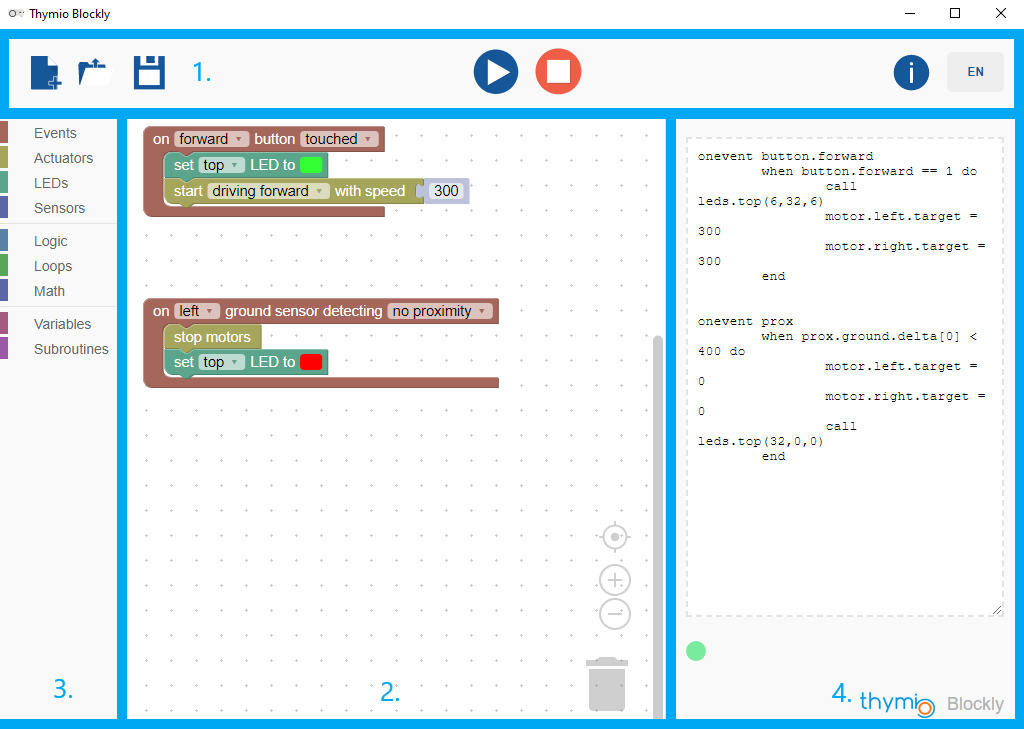
\includegraphics[scale=0.5]{./Blockly/blockly_window}\\
  Thymio Blockly window
\end{center}

The following figure displays a simple program. Once run the program listens to two different events. When the center button is pressed and when the front middle proximity sensor detects a wall. 
The first one will activate the two motors at the same speed, as to drive forward, and light the top LED to green. The second will stop the motors and turn the LED to red. \\
\begin{center}
  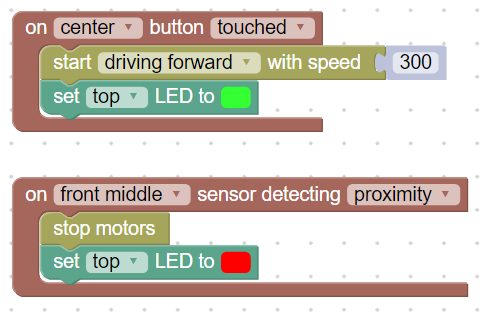
\includegraphics[scale=0.5]{./Blockly/forward_stop_wall}\\
  Basic program
\end{center}

Here we set a variable to control whether the \texttt{Thymio} is moving or not. This information is then used into a test when clicking the middle button, and either moving forward or stoping according to the result.
Two other events were added for the right and left buttons that are responsible to turn the robot.
\begin{center}
  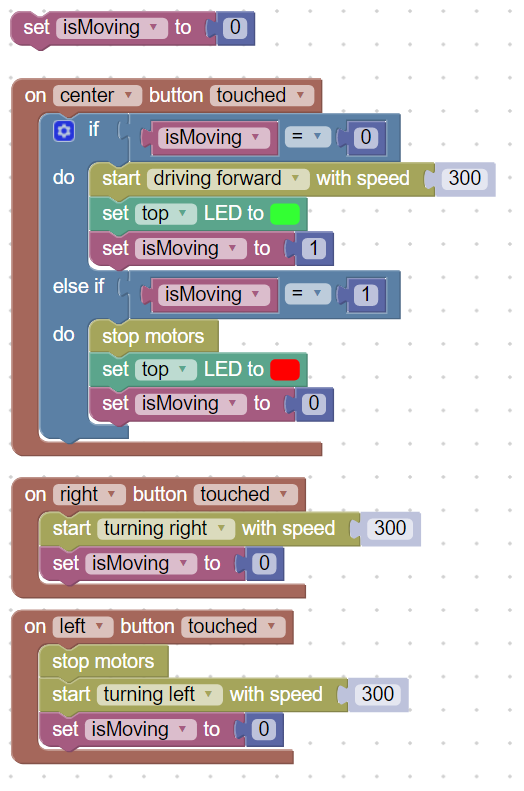
\includegraphics[scale=0.5]{./Blockly/advanced_program}\\
  More complex program
\end{center}

\section{Aseba}

For the \texttt{Aseba} possibility, we kindly recommend you to use the tutorials and examples that can be found on the \href{https://www.thymio.org/program/aseba/}{\texttt{Thymio} web page}.

\section{Scratch}

For the \texttt{Scratch} possibility, we kindly recommend you to use the tutorials and examples that can be found on the \href{https://www.thymio.org/program/scratch/}{\texttt{Thymio} web page}.

\chapter{Product Backlog}
\begin{longtable}{p{5mm}|p{2cm}|p{4cm}|p{1cm}|p{1cm}|p{1cm}|p{1cm}|p{15mm}}
  ID                     & Story Name & Story / Task Description & Priority & Est. Effort {[}h{]} & Update Effort {[}h{]} & Actual Effort{[}h{]} & Status                \\ \hline
  1 & Create Documentation & Develop and write the documentation & High & 16 & 16 & 16 & Done \\ 
  2 & Set up the Environment & Setting up and configuring the development environment & High & 12 & 12 & 12 & Done \\ 
  3 & Basic Learning & Learning and training of the different technology used later on & High & 44 & 58 & 58 & Done \\ 
  4 & Develop Playgrounds & Create playgrounds and function to generate meshes & High & 40 & 48 & 48 & Done \\ 
  5 & Update Documentation & Update existing documentation & High & 60 & 76 & 76 & Done \\
  6 & Architecture Implementation & Refactor the existing code into the designed architecture & High & 40 & 48 & 48 & Done\\ 
  7 & Web Deployement & Deploy the application on a webserver & High & 16 & 12 & 12 & Done \\ 
  8 & Basic UI & Implement a basic UI & Low & 8 & 8 & 8 & Done \\ 
  9 & Behavior Pipeline & Create pipeline to take .aesl file and translate/compile it into behavior in JavaScript for the Thymio II & High & 40 & 80 & 80 & Done \\ 
  10 & Phyisics Implementation & Implementation of Collisions for threejs Meshes & High & 20 & 16 & 16 & Done \\ 
  11 & Update Documentation & Update existing documentation & High & 20 & 20 & 20 & Done \\ 
  12 & Enhanced UI & Enhancement of the current UI & Low & 10 & [/] & {/} & To Do \\ 
  13 & Customizable Playgrounds & Implementation of a playground creator for users & High & 40 & 24 & 24 & Done \\ 
  14 & Update Documentation & Update existing documentation & High & 20 & 24 & 24 & Done \\ 
  15 & Enhanced Behavior Pipeline & Implement more sensors, action and event for Thymio II & High & {/} & {/} & {/} & To Do \\ 
  16 & Finish Documentation & Finish existing documentation & High & 80 & 88 & 88 & Done \\
  17 & Prepare Defense & Prepare the defense & High & 24 &  &  & To Do \\ 
\end{longtable}

\chapter{Sprint Backlog}
\section{First Sprint}
\textbf{2019-09-16 until 2019-10-07}
\begin{longtable}{p{5mm}|p{2cm}|p{4cm}|p{1cm}|p{1cm}|p{1cm}|p{1cm}|p{15mm}}
  ID                     & Story Name & Story / Task Description & Priority & Est. Effort {[}h{]} & Update Effort {[}h{]} & Actual Effort{[}h{]} & Status                \\ \hline
  1 & Create Documentation & Develop and write the documentation & High & 16 & 16 & 16 & Done \\ 
  1.1 & Template and Content & Choose a latex template and modify the content structure & High & 8 & 8 & 8 & Done \\ 
  1.2 & About Thymio & What is thymio and how does it work. & High & 8 & 8 & 8 & Done \\ 
  2 & Set up the Environment & Setting up and configuring the development environment & High & 12 & 12 & 12 & Done \\ 
  2.1 & GitHub & Create the project in GitHub and the Git environment & High & 4 & 4 & 4 & Done \\ 
  2.2 & Tools & Install Thymio Suite, NodeJS and download ThreeJS & High & 8 & 8 & 8 & Done \\ 
\end{longtable}

\section{Second Sprint}
\textbf{2019-10-07 until 2019-10-28}
\begin{longtable}{p{5mm}|p{2cm}|p{4cm}|p{1cm}|p{1cm}|p{1cm}|p{1cm}|p{15mm}}
  ID                     & Story Name & Story / Task Description & Priority & Est. Effort {[}h{]} & Update Effort {[}h{]} & Actual Effort{[}h{]} & Status                \\ \hline
  3 & Basic Learning & Learning and training of the different technology used later on & High & 44 & 58 & 58 & Done \\
  3.1 & threejs & Read documentation and examples, and practice & High & 16 & 20 & 20 & Done \\ 
  3.2 & JavaScript & Update and deepen knowledge  & High & 8 & 8 & 8 & Done \\ 
  3.3 & Thymio languages & Learning and using VPL, Blockly, Aseba and Scratch & Medium & 24 & 30 & 30 & Done \\ 
  4 & Develop Playgrounds & Create playgrounds and function to generate meshes & High & 40 & 48 & 48 & Done \\ 
  4.1 & Two Default Playgrounds & Generating two defalut playground to be choosen for the simulator & Medium & 12 & 12 & 12 & Done \\ 
  4.2 & Thymio Model & Create or load Thymio model & Medium & 4 & 4 & 4 & Done \\ 
  4.3 & Mesh Generation & Create function to generate meshes for the playgrounds & High & 24 & 32 & 32 & Done \\ 
  5 & Update Documentation & Update existing documentation & High & 60 & 12 & {/} & Done \\
  5.1 & Four supported languages & Descibe and initiate to VPL, Blockly, Aseba and Scratch & High & 24 & 12 & {/} & Done \\ 
\end{longtable}

\section{Third Sprint}
\textbf{2019-10-28 until 2019-11-15}
\begin{longtable}{p{5mm}|p{2cm}|p{4cm}|p{1cm}|p{1cm}|p{1cm}|p{1cm}|p{15mm}}
  ID                     & Story Name & Story / Task Description & Priority & Est. Effort {[}h{]} & Update Effort {[}h{]} & Actual Effort{[}h{]} & Status                \\ \hline
  5 & Update Documentation & Update existing documentation & High & 60 & 76 & 76 & Done \\
  5.1 & Four supported languages & Descibe and initiate to VPL, Blockly, Aseba and Scratch & High & 24 & 32 & 32 & Done \\ 
  5.2 & Backlogs & Create the Sprint and Project backlog & High & 12 & 16 & 16 & Done \\ 
  5.3 & Architecture & Create DCD, DM, PD, SD, SSD and proposition of architecture & High & 12 & 16 & 16 & Done \\
  5.4 & User Stories & Formulate the User Stories & Medium & 4 & 4 & 4 & Done \\ 
  5.5 & Risk Analysis & Create risk analysis & High & 8 & 8 & 8 & Done \\ 
  6 & Architecture Implementation & Refactor the existing code into the designed architecture & High & 40 & 48 & 48 & Done \\ 
  6.1 & Refactor Code & Refactor existing code into MVC Pattern & High & 20 & 44 & 44 & Done \\ 
  6.3 & Unit Testing & Write the JavaScript tests & High & 12 & {/} & {/} & To Do \\
  6.4 & JSDoc & Write the JavaScriptDoc & High & 8 & 4 & 4 & Done \\ 
  7 & Web Deployement & Deploy the application on a webserver & High & 16 & 12 & 12 & Done \\ 
  7.1 & Virtual Machine Setup & Set up the Virtual machine & High & 8 & 4 & 4 & Done \\ 
  7.2 & WebServer & Create WebServer and publish it on bfh network & High & 8 & 8 & 8 & Done \\
  8 & Basic UI & Implement a basic UI & Low & 8 & 8 & 8 & Done \\ 
  8.1 & Pages UI & Create three pages UI, one for each of the following index, simulation and creation pages & Low & 8 & 8 &  & Done \\
\end{longtable}

\section{Fourth Sprint}
\textbf{2019-11-15 until 2019-12-09}
\begin{longtable}{p{5mm}|p{2cm}|p{4cm}|p{1cm}|p{1cm}|p{1cm}|p{1cm}|p{15mm}}
  ID                     & Story Name & Story / Task Description & Priority & Est. Effort {[}h{]} & Update Effort {[}h{]} & Actual Effort{[}h{]} & Status                \\ \hline
  9 & Behavior Pipeline & Create pipeline to take .aesl file and translate/compile it into behavior in JavaScript for the Thymio II & High & 40 & 80 & 80 & Done \\ 
  10 & Phyisics Implementation & Implementation of Collisions for ThreeJS Meshes & High & 20 & 0 & {/} & To Do \\
  11 & Update Documentation & Update existing documentation & High & 20 & 20 & 20 & Done \\ 
\end{longtable}

\section{Fifth Sprint}
\textbf{2019-12-09 until 2019-12-30}
\begin{longtable}{p{5mm}|p{2cm}|p{4cm}|p{1cm}|p{1cm}|p{1cm}|p{1cm}|p{15mm}}
  ID                     & Story Name & Story / Task Description & Priority & Est. Effort {[}h{]} & Update Effort {[}h{]} & Actual Effort{[}h{]} & Status                \\ \hline
  12 & Enhanced UI & Enhancement of the current UI & Low & 10 & {/} & {/} & To Do \\ 
  10 & Phyisics Implementation & Implementation of Collisions for ThreeJS Meshes & High & 20 & 16 & 16 & Done \\
  13 & Customizable Playgrounds & Implementation of a playground creator for users & High & 40 & 24 & 24 & Done \\ 
  14 & Update Documentation & Update existing documentation & High & 20 & 24 & 24 & Done \\ 
\end{longtable}

\section{Sixth Sprint}
\textbf{2019-12-30 until 2020-01-17}
\begin{longtable}{p{5mm}|p{2cm}|p{4cm}|p{1cm}|p{1cm}|p{1cm}|p{1cm}|p{15mm}}
  ID                     & Story Name & Story / Task Description & Priority & Est. Effort {[}h{]} & Update Effort {[}h{]} & Actual Effort{[}h{]} & Status                \\ \hline
  15 & Enhanced Behavior Pipeline & Implement more sensors, action and event for Thymio II & High & {/} & {/} & {/} & To Do \\ 
  16 & Finish Documentation & Finish existing documentation & High & 80 & 88 & 88 & Done \\
  16.1 & Create Video & Create the video file & High & 16 & 16 & 16 & Done \\ 
  16.2 & Prepare Presentation Day & Create the poster and the presentation for the Presentation Day & High & 16 & 16 & 16 & Done \\
  16.3 & Write in the Book & Write the page for the Book & High & 8 & 4 & 4 & Done \\ 
  16.4 & Finish Writting Documentation & Terminate the writting part of the documentation & High & 32 & 44 & 44 & Done \\ 
  16.5 & Prepare to Submit & Check spelling mistake, check images, print it, put the project on a USB stick & High & 8 & 8 & 8 & Done\\ 
  17 & Prepare Defense & Prepare the defense & High & 24 &  &  & To Do \\ \hline
\end{longtable}

\chapter{Gantt Diagram}
%% TODO: make sure it's 100% visible

\begin{center}
  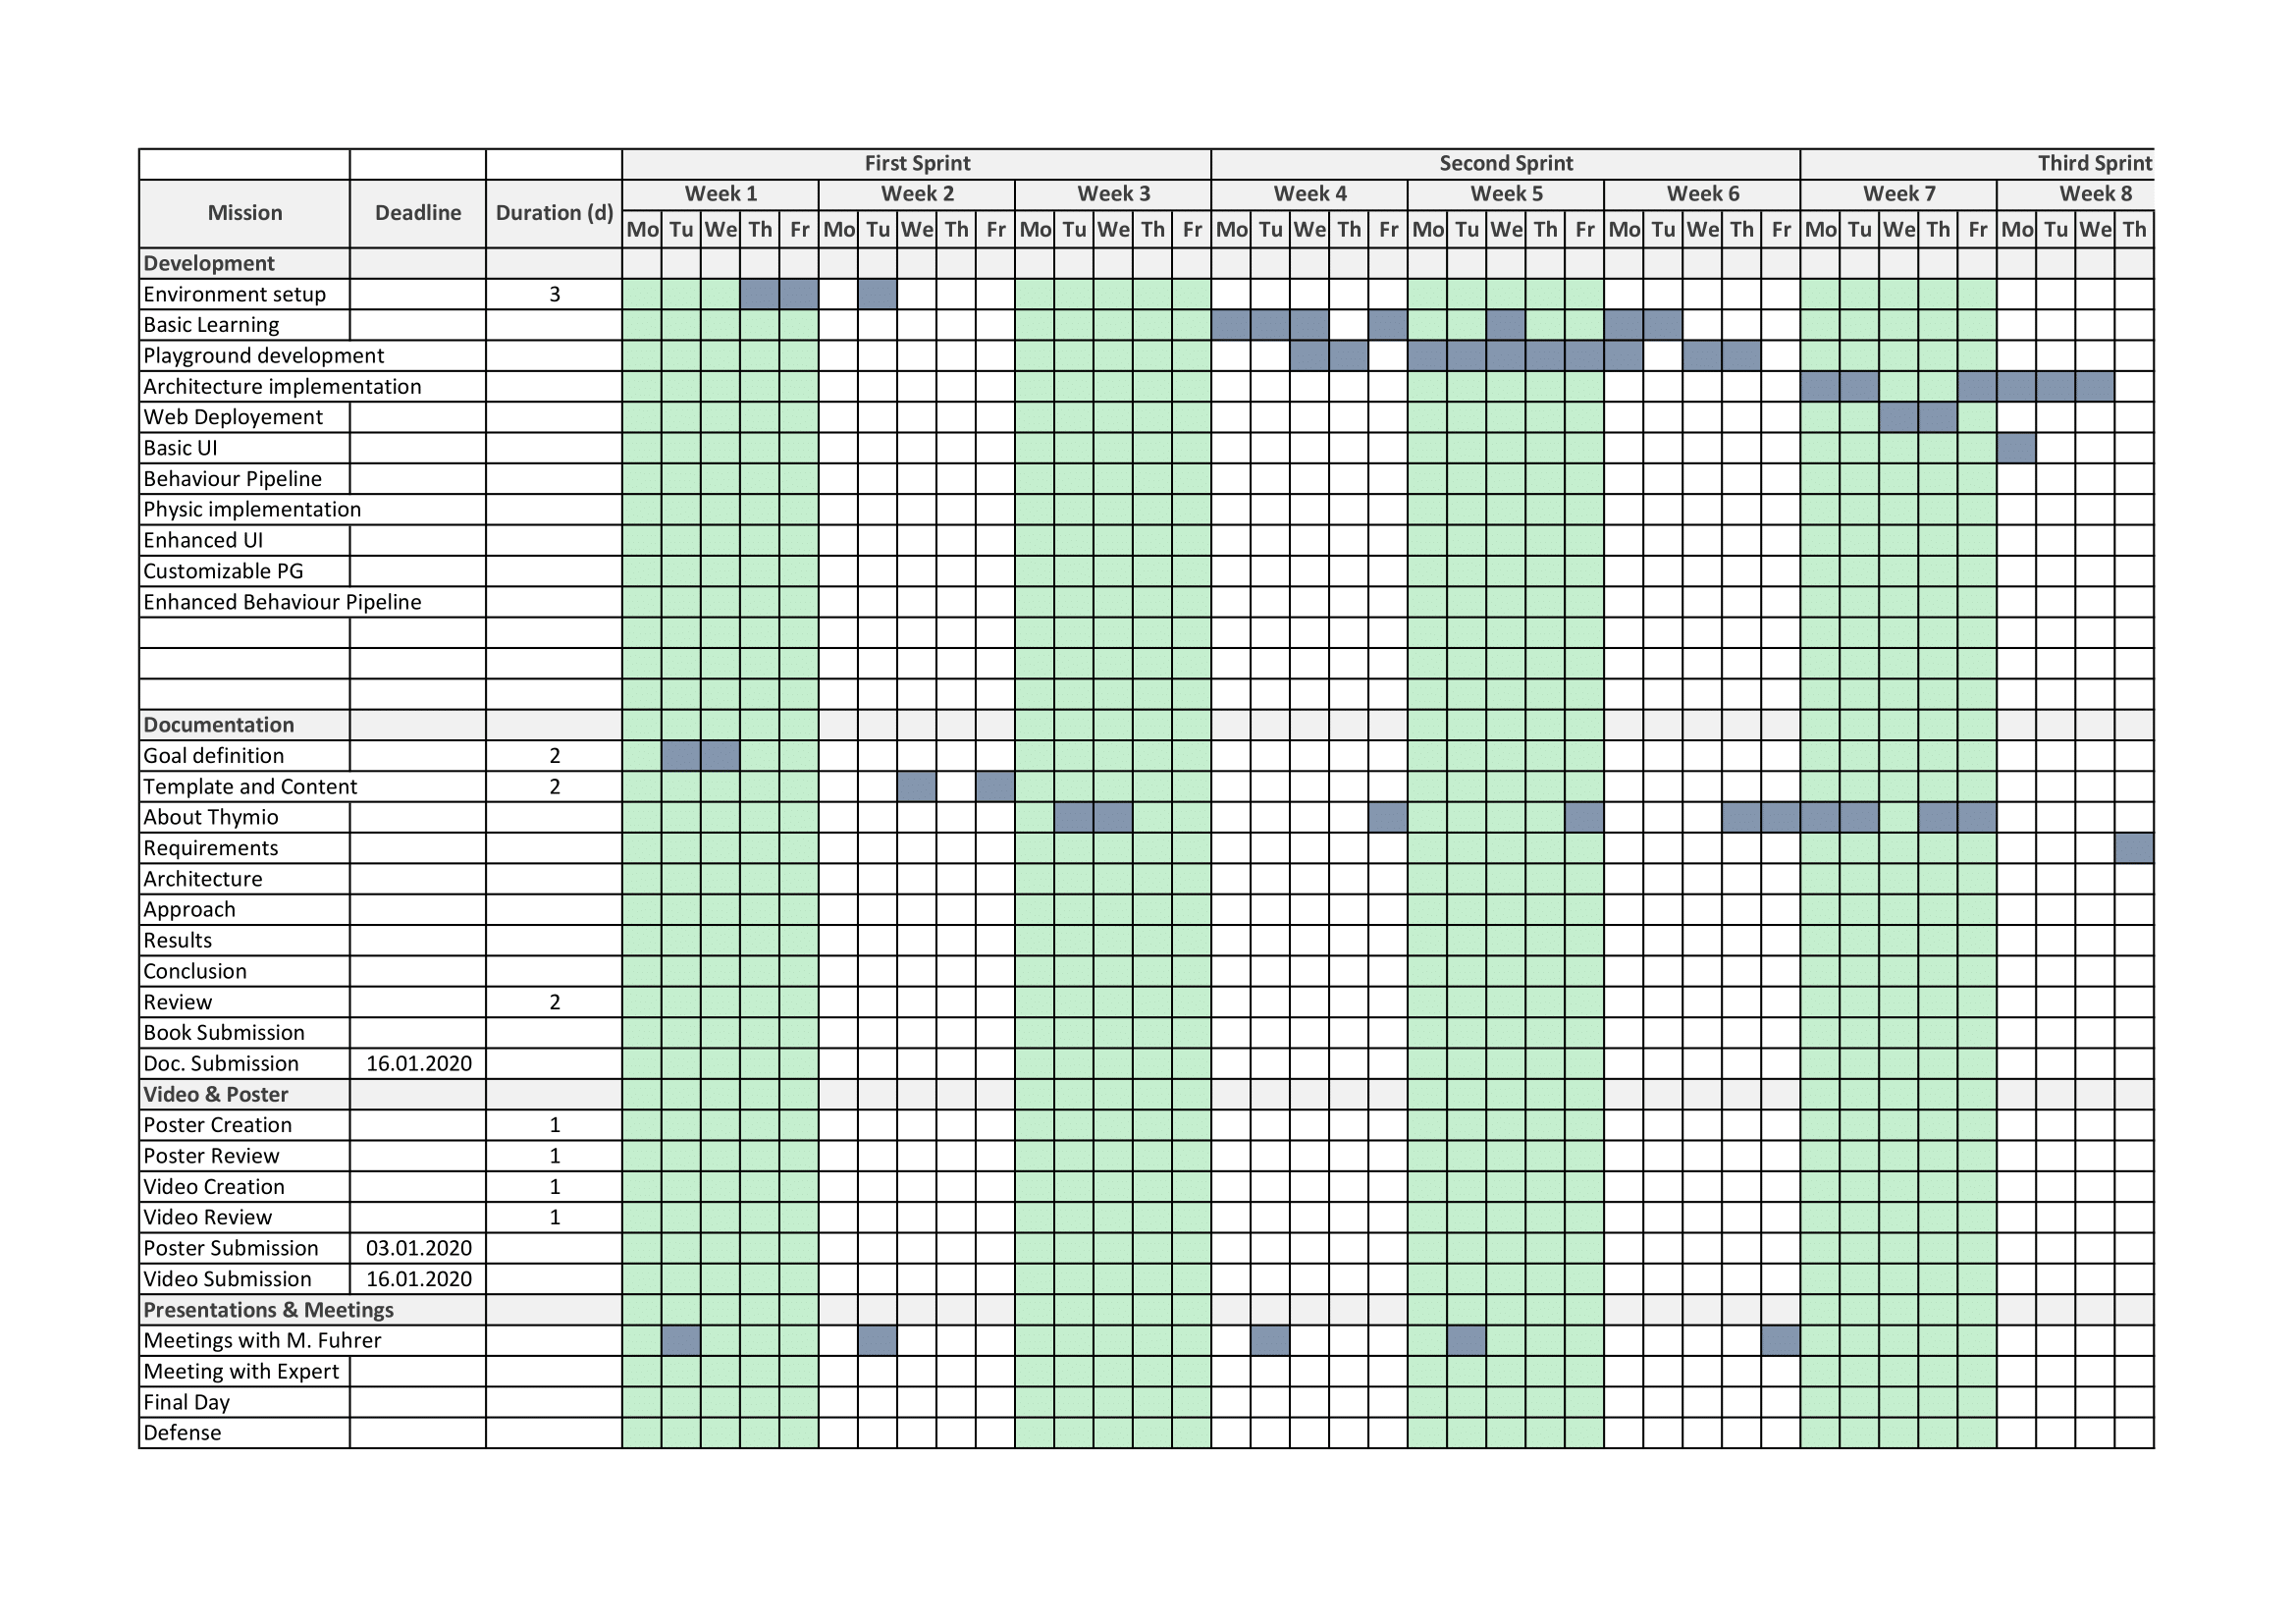
\includegraphics[scale = 0.31, angle=-90]{./Gantt-1}
\end{center}

\begin{center}
  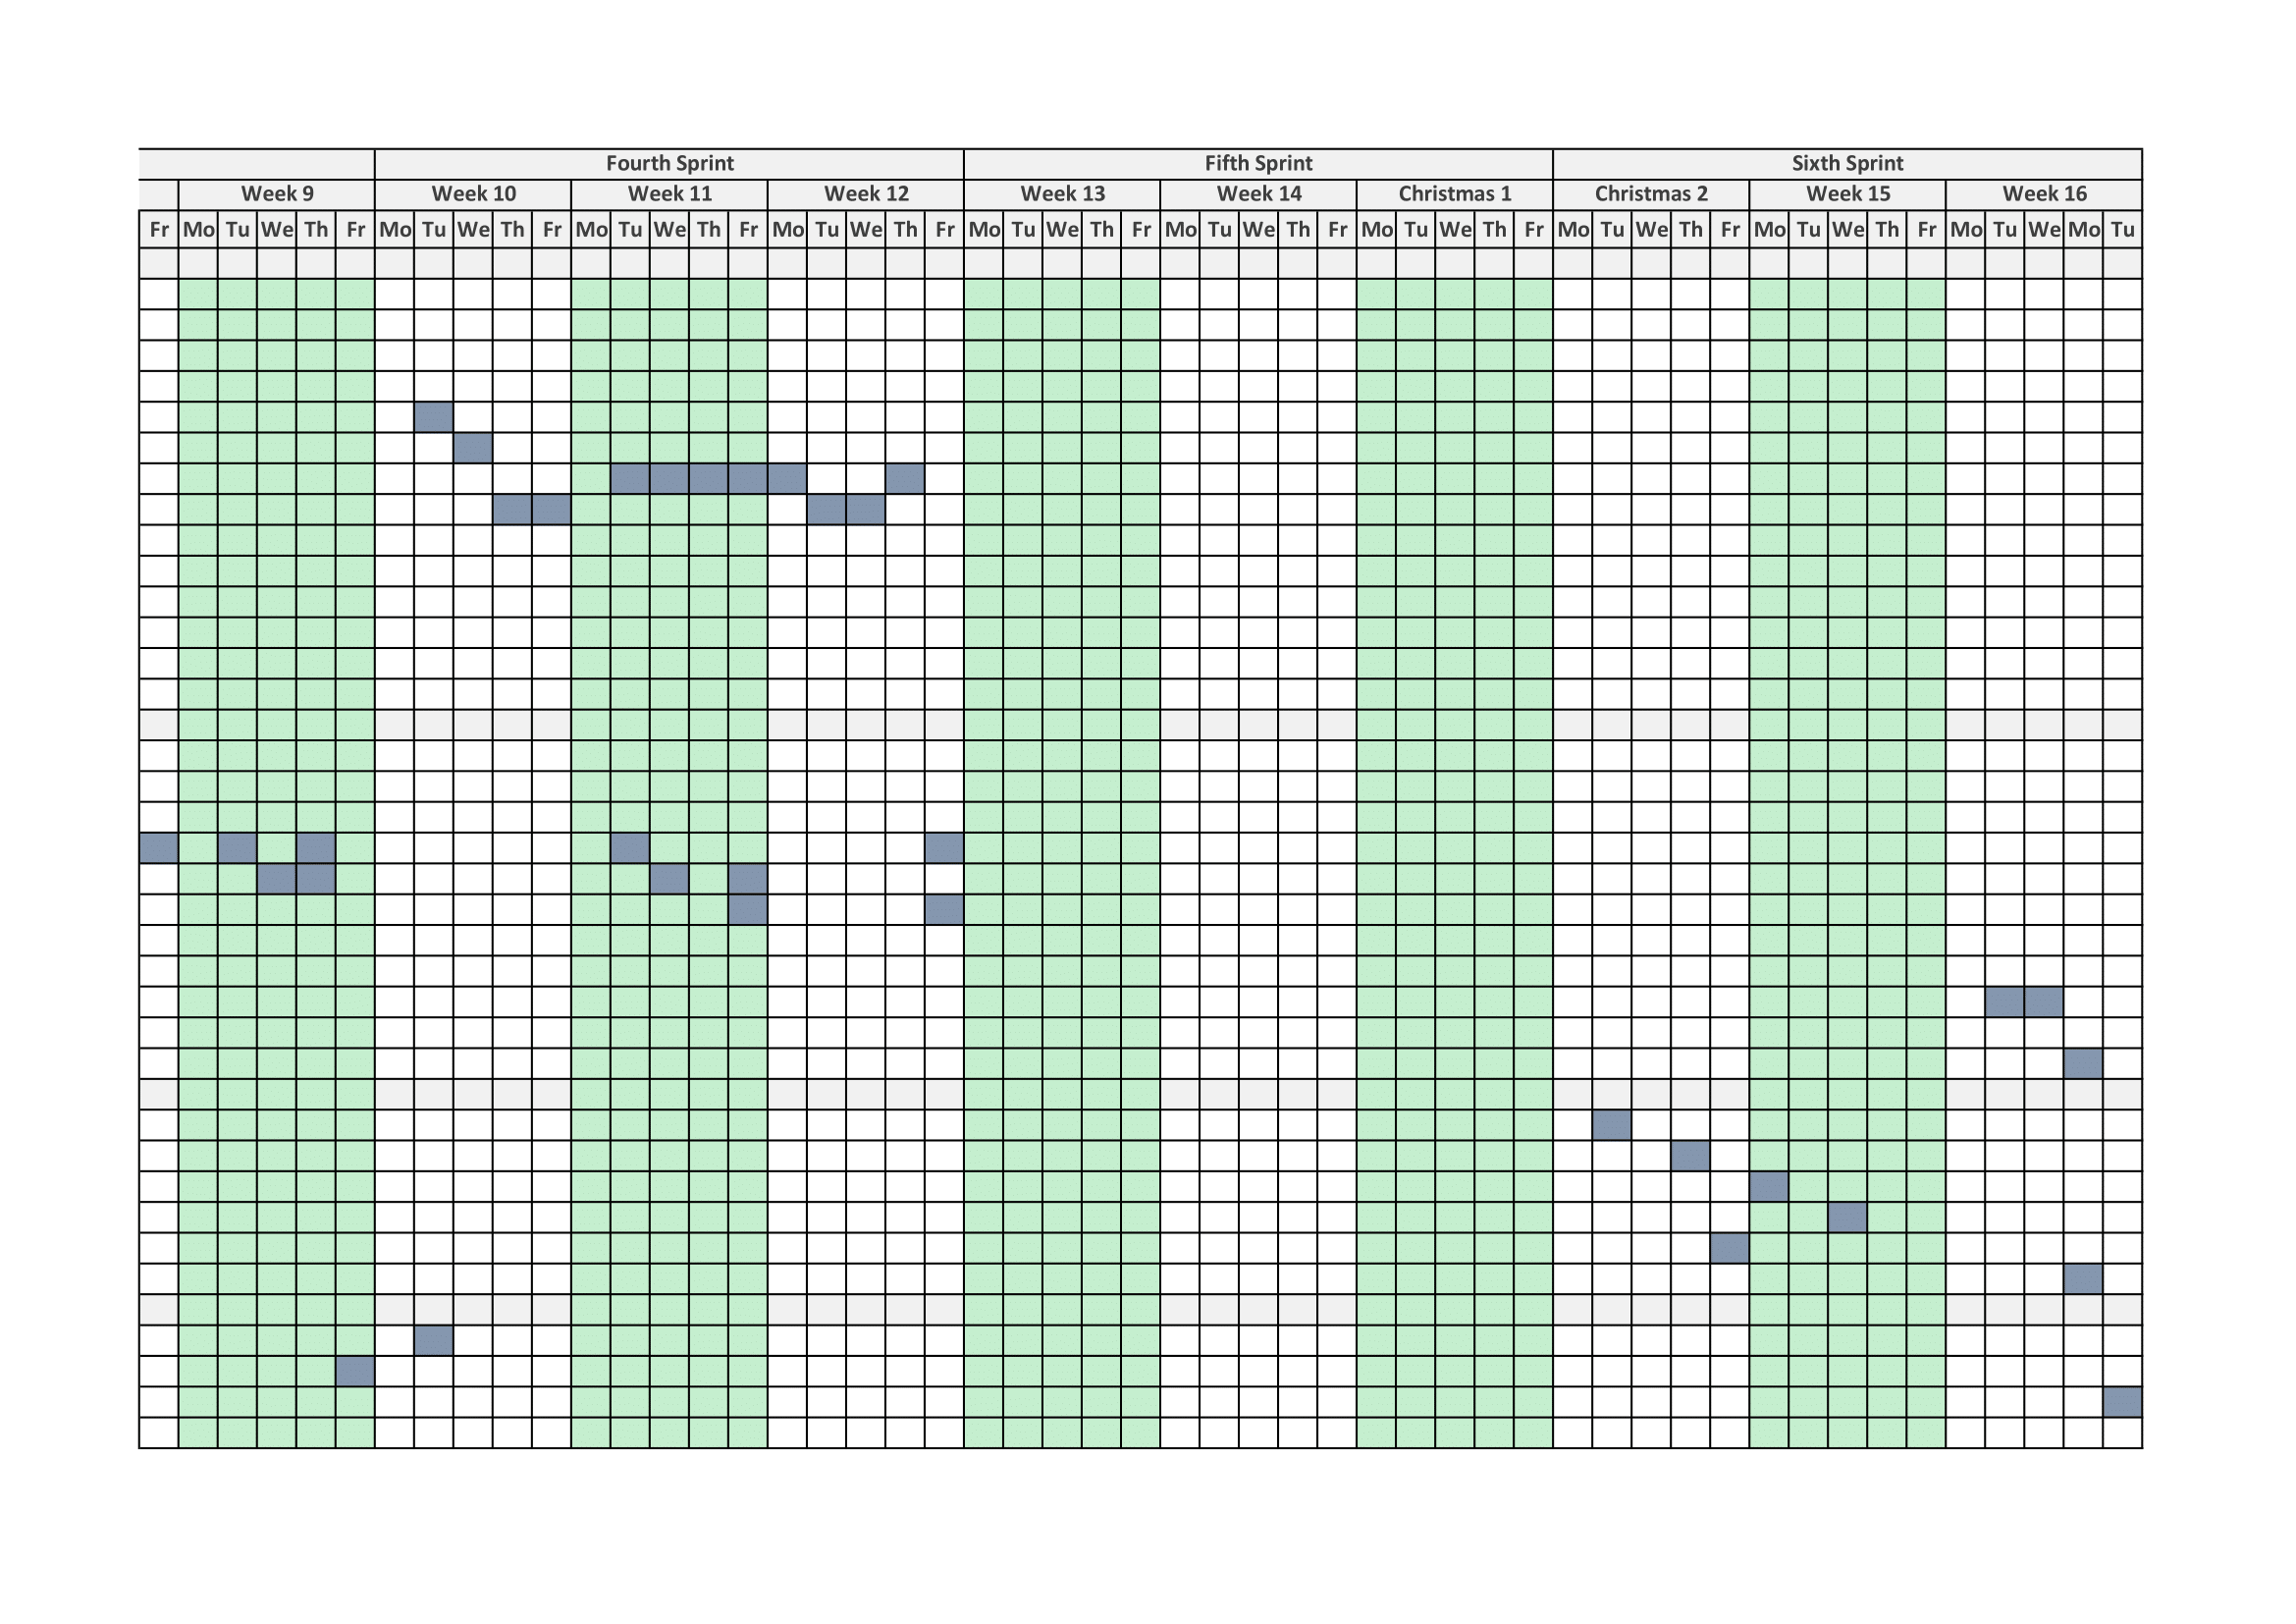
\includegraphics[scale = 0.31,  angle=-90]{./Gantt-2}
\end{center}

\chapter{Configuration}

\section{User Information}

On demand.

\section{Access the Windows Virtual Machine}

\begin{center}
  \begin{tabular}{|c|c|c|}
    \hline
     & Linux WM -ssh & Windows VM - rdp \\
    \hline
    Windows & Putty & Remote Desktop Connection \\
    \hline
    Linux & terminal & Remmina \\
    \hline
    MacOS & terminal & Microsoft Remote Desktop \\
    \hline
  \end{tabular}
\end{center}

See the link below for more information and links. It requires to be inside the bfh networkd to access it
\url{https://intranet.bfh.ch/TI/fr/Studium/Bachelor/Informatik/Tools/VMsHowto/Pages/default.aspx?k=vm}

\section{First Configuration of XAMPP}
The configuration of XAMPP is very basic. The steps done during the setup of the IIS Manager at \ref{webserver}, concerning forwarding and firewall, should still be followed. First, we need to download and install it. It can be found under this link: \url{https://www.apachefriends.org/index.html} . Afterward, it is needed to travel through the folder of the application until the folder 
\texttt{htdocs}. This is where the default placeholder files was stored. There, we put them into a new default folder and instead added our content in this folder. It should not be forgotten to take the .webconfig file from the \ref{webserver} section.

\chapter{Meetings}

\begin{tabular}{ | m{3cm} | m{10cm} | }
  \hline
  Date & Content \\
  \hline
  17.09.2019 & \textbf{Kick Off meeting}\\
  & - Documentation/Management\\
  & - Technology to use : ThreeJS and Typescript\\
  & - Setting up the goals\\
  \hline
  24.09.2019 & \textbf{Second meeting} \\
  & - Documentation language : English \\
  & - Thymio model \\
  & - Base talk about risk management \\
  \hline
  08.10.2019 & \textbf{Third meeting}\\
  & Workplace\\
  & - Discussion on the choice of Windows as the Virtual Machine \\
  & - Create a configuration file with the information of the VM \\
  & - And an architecture proposal \\
  \hline
  15.10.2019 & \textbf{Fourth meeting} \\
  & - Which shapes and meshes should the user be able to create for his own custom playground \\
  & - Problems with webserver, has to be accessible from outside the vm, so maybe switching from windosw to linux \\
  & - Talk about the problem of thymio suite, where the software only allows the user to create programs if a physical or a simulated one is plugged in \\
  \hline
  25.10.2019 & \textbf{Fifth meeting} \\
  & - Discussed using a Finite state machine to handle the events, but it may be too rigid so a non-deterministic finite state machine was the possible solution we came with \\
  & - First little talk about the meeting with the expert, report\\
  \hline
  19.11.2019 & \textbf{Sixth meeting} \\
  & \\
  \hline
  07.12.2019 & \textbf{Seventh meeting} \\
  & \\
  \hline
  19.12.2019 & \textbf{Eighth meeting} \\
  & - Documentation review\\
  & - What to hand in to the secretariat and to Mr. Fuhrer\\
  \hline
  07.01.2020 & \textbf{Ninth meeting} \\
  & - Documentation state\\
  & - Latex commands\\
  & - Final day and defense talk\\
  \hline
  14.01.2020 & \textbf{Tenth meeting} \\
  & - Latex commands\\
  & - Organizational questions\\
 \hline
\end{tabular}

\chapter{Problems encountered}
\begin{itemize}
  \item javascript not refreshing properly due to cache -> disable cache
  \item 3d Model not loaded on the webserver -> first tried to change the directory, then mixed two solution. 
        Had to create a web.config file and add file extension for .mtl and .obj.
        https://stackoverflow.com/questions/41245938/web-server-cannot-find-mtl-file
        https://stackoverflow.com/questions/16097580/three-js-loading-obj-error-in-azure-but-not-locally
  \item shadow not rendering on plane of all playgrounds
  \item javascript file not found on server, net::ERR\textunderscore ABORTED 404 (Not Found) => first solution (working partially) was to add a IIS\textunderscore IUSRS.
  \item Thymio Blockly has trouble loading saved files. Using the software I was not able to load any .aesl file previously created with it, but I could load them if I used the index.html one.
  \item Thymio model not always loading correctly -> Load one at the start of the page and reset its position/rotation upon change of playground.
  \item problem with dat.gui, it was creating a new creator view so the creator was not accessible -> decided to use html buttons instead
  \item c++ to javascript
\end{itemize}



\includegraphics[width=\textwidth]{pdf/Declaration_of_authonomy.pdf}

%% Print the bibibliography and add the section to the table of content
\printbibliography[heading=bibintoc]

\end{document}
